% ---------------------------------------------------------------------------------------------------------------
% TEMPLATE PARA TRABALHO DE CONCLUSÃO DE CURSO
% Universidade Tecnológica Federal do Paraná - UTFPR
% Customização da classe abnTeX2 (http://www.abntex.net.br/) para as normas da UTFPR
%
% Autores: Diego Marczal
% 	       Michael Vornes <https://github.com/mvornes>
% Adaptação (DACOM-CP): Silvio Ricardo Rodrigues Sanches
%
%----------------------------------------------------------------------------------------------------------------
% Codificação: UTF-8
% LaTeX:  abnTeX2          
% ---------------------------------------------------------------------------------------------------------------


% CARREGA CLASSE PERSONALIZADA DA UTFPR--------------------------------------------------------------------------
\documentclass[%twoside,                   % Impressão em frente e verso
    	        oneside,                   % Impressão apenas frente
]{configuracoes/utfpr-abntex2}


% INCLUI ARQUIVOS DE CONFIGURAÇÕES-------------------------------------------------------------------------------
% REFERÊNCIAS------------------------------------------------------------------
\usepackage[%
    alf,
    abnt-emphasize=bf,
    bibjustif,
    recuo=0cm,
    abnt-url-package=url,       % Utiliza o pacote url
    abnt-refinfo=yes,           % Utiliza o estilo bibliográfico abnt-refinfo
    abnt-etal-cite=3,
    abnt-etal-list=3,
    abnt-thesis-year=final
]{abntex2cite}                  % Configura as citações bibliográficas conforme a norma ABNT

% PACOTES----------------------------------------------------------------------
\usepackage[utf8]{inputenc}                                 % Codificação do documento
\usepackage[T1]{fontenc}                                    % Seleção de código de fonte
\usepackage{booktabs}                                       % Réguas horizontais em tabelas
\usepackage{color, colortbl}                                % Controle das cores
\usepackage{float}                                          % Necessário para tabelas/figuras em ambiente multi-colunas
\usepackage{graphicx}                                       % Inclusão de gráficos e figuras
\usepackage{icomma}                                         % Uso de vírgulas em expressões matemáticas
\usepackage{indentfirst}                                    % Indenta o primeiro parágrafo de cada seção
\usepackage{microtype}                                      % Melhora a justificação do documento
\usepackage{multirow, array}                                % Permite tabelas com múltiplas linhas e colunas
\usepackage{subeqnarray}                                    % Permite subnumeração de equações
\usepackage{lastpage}                                       % Para encontrar última página do documento
\usepackage{verbatim}                                       % Permite apresentar texto tal como escrito no documento, ainda que sejam comandos Latex
\usepackage{amsfonts, amssymb, amsmath}                     % Fontes e símbolos matemáticos
\usepackage[algoruled, portuguese]{algorithm2e}             % Permite escrever algoritmos em português
%\usepackage[scaled]{helvet}                                % Usa a fonte Helvetica
\usepackage{times}                                          % Usa a fonte Times
%\usepackage{palatino}                                      % Usa a fonte Palatino
%\usepackage{lmodern}                                       % Usa a fonte Latin Modern
\usepackage[bottom]{footmisc}                               % Mantém as notas de rodapé sempre na mesma posição
\usepackage{ae, aecompl}                                    % Fontes de alta qualidade
\usepackage{latexsym}                                       % Símbolos matemáticos
\usepackage{lscape}                                         % Permite páginas em modo "paisagem"
%\usepackage{picinpar}                                      % Dispor imagens em parágrafos
%\usepackage{scalefnt}                                      % Permite redimensionar tamanho da fonte
\usepackage{subfig}                                        % Posicionamento de figuras
%\usepackage{upgreek}                                       % Fonte letras gregas
\usepackage{graphicx}                                       % Tabelas
\usepackage[table,xcdraw]{xcolor}
% Redefine a fonte para uma fonte similar a Arial (fonte Helvetica)
\renewcommand*\familydefault{\sfdefault}
% CONFIGURAÇÕES DE APARÊNCIA DO PDF FINAL--------------------------------------
\makeatletter
\hypersetup{%
    portuguese,
    colorlinks=true,   % true: "links" coloridos; false: "links" em caixas de texto
    linkcolor=blue,    % Define cor dos "links" internos
    citecolor=blue,    % Define cor dos "links" para as referências bibliográficas
    filecolor=blue,    % Define cor dos "links" para arquivos
    urlcolor=blue,     % Define a cor dos "hiperlinks"
    breaklinks=true,
    pdftitle={\@title},
    pdfauthor={\@author},
    pdfkeywords={abnt, latex, abntex, abntex2}
}
\makeatother

% ALTERA O ASPECTO DA COR AZUL--------------------------------------------------
\definecolor{blue}{RGB}{41,5,195}

% REDEFINIÇÃO DE LABELS---------------------------------------------------------
\renewcommand{\algorithmautorefname}{Algoritmo}
\def\equationautorefname~#1\null{Equa\c c\~ao~(#1)\null}

% CRIA ÍNDICE REMISSIVO---------------------------------------------------------
\makeindex

% HIFENIZAÇÃO DE PALAVRAS QUE NÃO ESTÃO NO DICIONÁRIO---------------------------
\hyphenation{%
    qua-dros-cha-ve
    Kat-sa-gge-los
}



% INCLUI ARQUIVOS DO TRABALHO DE CONCLUSÃO DE CURSO (PRÉ-TEXTUAIS, TEXTUAIS, PÓS-TEXTUAIS)-----------------------

% INSERE CAPA E FOLHA DE ROSTO
% CAPA---------------------------------------------------------------------------------------------------

% ORIENTAÇÕES GERAIS-------------------------------------------------------------------------------------
% Caso algum dos campos não se aplique ao seu trabalho, como por exemplo,
% se não houve coorientador, apenas deixe vazio.
% Exemplos: 
% \coorientador{}
% \departamento{}

% DADOS DO TRABALHO--------------------------------------------------------------------------------------
\titulo{MODELO DE DESCRIÇÃO DE TEXTURAS EM IMAGENS BASEADO EM ÁRVORES GERADORAS MÍNIMAS}
\titleabstract{TEXTURE DESCRIPTION MODEL IN IMAGES BASED ON MINIMUM SPANNING TREES}
\autor{Felipe Seolin Bento}
\autorcitacao{BENTO, Felipe Seolin} % Sobrenome em maiúsculo
\local{Cornélio Procópio}
\data{2021}

% NATUREZA DO TRABALHO-----------------------------------------------------------------------------------
% Opções: 
% - Trabalho de Conclusão de Curso (se for Graduação)
% - Dissertação (se for Mestrado)
% - Tese (se for Doutorado)
% - Projeto de Qualificação (se for Mestrado ou Doutorado)
\projeto{Trabalho de Conclusão de Curso}

% TÍTULO ACADÊMICO---------------------------------------------------------------------------------------
% Opções:
% - Bacharel ou Tecnólogo (Se a natureza for Trabalho de Conclusão de Curso)
% - Mestre (Se a natureza for Dissertação)
% - Doutor (Se a natureza for Tese)
% - Mestre ou Doutor (Se a natureza for Projeto de Qualificação)
\tituloAcademico{Bacharel em Engenharia de Software}

% ÁREA DE CONCENTRAÇÃO E LINHA DE PESQUISA---------------------------------------------------------------
% Se a natureza for Trabalho de Conclusão de Curso, deixe ambos os campos vazios
% Se for programa de Pós-graduação, indique a área de concentração e a linha de pesquisa
\areaconcentracao{}
\linhapesquisa{}

% DADOS DA INSTITUIÇÃO-----------------------------------------------------------------------------------
% Se a natureza for Trabalho de Conclusão de Curso, coloque o nome do curso de graduação em "programa"
% Formato para o logo da Instituição: \logoinstituicao{<escala>}{<caminho/nome do arquivo>}
\instituicao{Universidade Tecnológica Federal do Paraná}
\departamento{Departamento Acadêmico de Computação}
\programa{Curso de Bacharelado em Engenharia de Software}
\logoinstituicao{0.2}{dados/figuras/logo-instituicao.png} 

% DADOS DOS ORIENTADORES---------------------------------------------------------------------------------
\orientador{Prof. Dr. Pedro Henrique Bugatti}
%\orientador[Orientadora:]{Nome da orientadora}
\instOrientador{Universidade Tecnológica Federal do Paraná}

%\coorientador{Prof. Dr. Alexandre Rômulo Moreira Feitosa}
%\coorientador[Coorientadora:]{Nome da coorientadora}
%\instCoorientador{Universidade Tecnológica Federal do Paraná}

% FOLHA DE ROSTO--------------------------------------------------------------------------------------------------------

% TRABALHO DE CONCLUSÃO DE CURSO
 \preambulo{{\imprimirprojeto} apresentado ao {\imprimirprograma} da {\imprimirinstituicao}, como requisito parcial para a obtenção do título de {\imprimirtituloAcademico}.}

% DISSERTAÇÃO DE MESTRADO
% \preambulo{{\imprimirprojeto} apresentada ao Programa de \mbox{Pós-graduação} da {\imprimirinstituicao}, como requisito parcial para obtenção do título de {\imprimirtituloAcademico}.}

% TESE DE DOUTORADO
% \preambulo{{\imprimirprojeto} apresentada ao Programa de \mbox{Pós-graduação} da {\imprimirinstituicao}, como requisito parcial para a obtenção do título de {\imprimirtituloAcademico}.}

% PROJETO DE QUALIFICAÇÃO DE MESTRADO OU DOUTORADO
%\preambulo{{\imprimirprojeto} apresentado ao Programa de \mbox{Pós-graduação} da {\imprimirinstituicao}, como requisito parcial para a obtenção do título de {\imprimirtituloAcademico}.}

% OBSERVAÇÕES-----------------------------------------------------------------------------------------------------------
% Altere este arquivo APENAS comentando as linhas que não se aplicam ao tipo de trabalho acadêmico desejado.


\begin{document}

\pretextual
% Comando para imprimir Capa
\imprimircapa
% Comando para imprimir Folha de rosto
\imprimirfolhaderosto{}
% INSERE ELEMENTOS PRÉ-TEXTUAIS

% Resumo em Português
% RESUMO--------------------------------------------------------------------------------

\begin{resumo}[RESUMO]
\begin{SingleSpacing}

% Não altere esta seção do texto--------------------------------------------------------
\imprimirautorcitacao. \imprimirtitulo. \imprimirdata. \pageref {LastPage} f. \imprimirprojeto\ – \imprimirprograma, \imprimirinstituicao. \imprimirlocal, \imprimirdata.\\
%---------------------------------------------------------------------------------------

O mundo está repleto de imagens, as quais possuem uma vasta quantidade de dados que podem ser processados de formas distintas. No contexto de imagens digitais, o seu processamento pode auxiliar diversas áreas como saúde, astronomia, agroindústria, entre outras. A descrição de uma imagem é uma etapa importante dentro do processamento digital de imagens, pois é responsável por identificar texturas, cores ou formas. Para isto, há uma tendência de estudos que buscam diferentes abordagens para algoritmos que descrevam objetos dentro de uma imagem da melhor forma possível. Neste sentido, este trabalho apresenta uma nova abordagem para tal etapa de processamento de imagens digitais, baseada em estudo de grafos, mais especificamente em árvores geradoras mínimas. Assim, obtendo como resultado a análise, discussão e validação deste novo algoritmo extrator. O algoritmo desenvolvido liga todos os \textit{pixels} de uma imagem, de forma a caracterizar vizinhança oito, em seguida pondera todas as arestas a partir do módulo da diferença entre os \textit{pixels}, encontra a árvore geradora mínima e a partir dos valores das arestas calcula algumas medidas de forma a montar um vetor de características. Por fim, pode-se afirmar que ao comparar os resultados do algoritmo proposto com outros já consolidados na literatura e submeter a testes em diferentes cenários, o algoritmo se mostrou eficaz na maioria das vezes, apresentando acurácias próximas aos comparados e até mesmo melhores em determinadas situações.
\\

\textbf{Palavras-chave}: Imagem.  Textura. Processamento Digital de Imagens. Descrição de Imagens. Árvore Geradora Mínima.

\end{SingleSpacing}
\end{resumo}

% OBSERVAÇÕES---------------------------------------------------------------------------
% Altere o texto inserindo o Resumo do seu trabalho.
% Escolha de 3 a 5 palavras ou termos que descrevam bem o seu trabalho 

% Resumo em Inglês
% ABSTRACT--------------------------------------------------------------------------------

\begin{resumo}[ABSTRACT]
\begin{SingleSpacing}

% Não altere esta seção do texto--------------------------------------------------------
\imprimirautorcitacao. \imprimirtitleabstract. \imprimirdata. \pageref {LastPage} f. \imprimirprojeto\ – \imprimirprograma, \imprimirinstituicao. \imprimirlocal, \imprimirdata.\\
%---------------------------------------------------------------------------------------

The world is full of images, which contain a vast amount of data that can be processed in different ways. In the context of digital images, its processing can help different areas such as health, astronomy, agribusiness, among others. The description of an image is an important step in digital image processing, as it is responsible for identifying textures, colors or shapes. For this, there is a trend of studies that seek different approaches to algorithms that describe objects within an image in the best possible way. In this sense, this work presents a new approach for this stage of digital image processing, based on the study of graphs, more specifically on minimal spanning trees. Thus, obtaining as a result the analysis, discussion and validation of this new extractor algorithm. The algorithm connects all the pixels of an image, in order to characterize neighborhood eight, then it weights all the edges from the modulus of the difference between the pixels, finds the minimum spanning tree and from the edge values it calculates some shape measures to assemble a vector of features. Finally, it can be said that when comparing the results of the proposed algorithm with others already consolidated in the literature and submitting to tests in different scenarios, the algorithm proved to be effective most of the time, presenting accuracy close to those compared and even better in certain situations.
\\

\textbf{Keywords}: Image. Texture. Digital Image Processing. Images Description. Minimum Spanning Tree.

\end{SingleSpacing}
\end{resumo}

% OBSERVAÇÕES---------------------------------------------------------------------------
% Altere o texto inserindo o Abstract do seu trabalho.
% Escolha de 3 a 5 palavras ou termos que descrevam bem o seu trabalho 

% Lista de Figuras
% Lista de Figuras----------------------------------------------------------------

\pdfbookmark[0]{\listfigurename}{lof}
\listoffigures*
\cleardoublepage

% OBSERVAÇÕES---------------------------------------------------------------------
% Este arquivo não precisa de ser alterado, pois a lista é gerada automaticamente.

% Lista de Tabelas
% LISTA DE TABELAS-------------------------------------------------------------

\pdfbookmark[0]{\listtablename}{lot}
\listoftables*
\cleardoublepage

% OBSERVAÇÕES-------------------------------------------------------------------
% Este arquivo não precisa ser alterado, pois a lista é gerada automaticamente.

% Lista de Abreviaturas e Siglas
% LISTA DE ABREVIATURAS E SIGLAS----------------------------------------------------------

\begin{siglas}
    \item[BIC] \textit{Border/Interior Pixel Classification}
    \item[CGH] \textit{Global Color Histogram}
    \item[GUI] \textit{Graphical User Interface}
    \item[LBP] \textit{Local Binary Patterns}
    \item[LHC] \textit{Local Color Histogram}
    \item[MST] \textit{Minimum Spanning Trees}
    \item[OpenCV] \textit{Open Source Computer Vision Library}
    \item[TCC] Trabalho de Conclusão de Curso
    \item[UTFPR] Universidade Tecnológica Federal do Paraná
    \item[PNG] \textit{Portable Network Graphics}
    \item[VisTex] Vision Texture
\end{siglas}

% OBSERVAÇÕES-----------------------------------------------------------------------------
% Altere a lista acima para definir os acrônimos e siglas utilizados neste trabalho

% Sumário
% SUMÁRIO----------------------------------------------------------------------

\renewcommand{\contentsname}{SUMÁRIO}

\pdfbookmark[0]{\contentsname}{toc}
\tableofcontents*
\cleardoublepage

% OBSERVAÇÕES-------------------------------------------------------------------
% Este arquivo não precisa ser alterado, pois o sumário é gerado automaticamente.


% INSERE ELEMENTOS TEXTUAIS
\textual
% Introdução
% INTRODUÇÃO-------------------------------------------------------------------

\chapter{INTRODUÇÃO}
\label{chap:introducao}

\par A visão é o mais avançado dos sentidos humanos, por consequência, as imagens são elementos de grande importância. No entanto, a espécie humana possui uma limitação quanto a captação de imagens, tendo acesso apenas à camada visível do espectro eletromagnético. Limitação esta que equipamentos da área de processamento de imagens não possuem pois alcançam dos raios gama às ondas rádio do espectro \cite{valencca2011monitorizaccao}.

\par O mundo está repleto de imagens, as quais possuem uma vasta quantidade de dados que podem ser encontrados e processados de formas distintas. Isto não é diferente quando se trata de imagens digitais, pois estas representam uma quantia significativa de medições existentes. Porém, para imagens de ressonância magnéticas, tomografias, observações astronômicas e outras se tornarem compreensíveis é preciso extrair informações: ação possível devido ao processamento de imagens digitais \cite{ScikitImage}.

\par Sendo assim, o processamento de imagens digitais tem como principal objetivo o tratamento de tais dados das imagens \cite{ScikitImage}. Para \citeonline{Gonzalez2009}, esta área não diz respeito apenas à entrada de uma imagem que é processada e resulta em outra, mas também ao reconhecimento de determinados atributos, como cores e texturas, além da capacidade de uma máquina de reconhecer padrões e até mesmo aprender com as informações presentes.

\par \citeonline{jarbas-analise-textura} ainda acrescentam que o processamento de imagem possui grande importância na computação visual, sendo a textura caracterizada como um dos elementos principais e essenciais para alguns campos como: detecção de objetos, recuperação de imagens, sensoriamento remoto entre outros. 

\par Apesar disto, a textura não possui uma definição exata na literatura. Alguns a caracterizam como a repetição de um modelo na imagem com pequenas variações. Outros, no entanto, dizem que até mesmo a ausência de padrões é capaz de caracterizar uma textura. Uma das definições mais bem aceitas, diz que textura corresponde a padrões visuais complexos que são formados por entidades ou sub-padrões, com características específicas como: tamanho, brilho e outras \cite{jarbas-color-texture}. 

\par Atualmente, a textura tem se tornado um atributo de descrição muito estudado e fonte de diversas pesquisas. Apesar de já existirem métodos consolidados, há uma tendência de novos estudos que buscam abordagens diferentes, sejam por matrizes de co-ocorrência, análise espectral ou outros \cite{jarbas-analise-textura}. 

\par Posto isto, o objetivo deste trabalho é desenvolver uma nova abordagem para a descrição de texturas em imagens digitais, sendo baseada em árvores geradoras mínimas, também conhecidas como \textit{minimum spanning trees} (MST). Assim, sendo capaz de contribuir para esta área, a partir das descobertas feitas pela análise de seu desempenho, além de preencher uma lacuna de conhecimento existente sobre a utilização da MST para a descrição de texturas.


\section{PROBLEMA}
\label{sec:problema}

\par Atualmente podemos encontrar diversos algoritmos de descrição de imagens, tais quais podem se dividir em descrição de: cor, textura e/ou forma. Para descrição de cor há por exemplo: \textit{Border/Interior Pixel Classification} (BIC) \cite{bic-stehling2002compact}, \textit{Global Color Histogram} (CGH) \cite{cgh-stricker1995similarity} e \textit{Local Color Histogram} (LHC) \cite{lhc-smith1996local}. Já para a descrição de textura existem as seguintes técnicas: Matrizes \textit{Run-length}, \textit{Local Binary Patterns} (LBP) \cite{lbp-guo2010rotation} e  Descritores de Haralick \cite{haralick1973textural}. Por fim, para se descrever formas há: Assinatura, Código da cadeia, segundo Freeman, Momentos, segundo Ming-Kuei Hu, entre outros \cite{Gonzalez2009}.
\par Assim como provado por \citeonline{jarbas-color-texture}, novos algoritmos podem ser capazes de extrair propriedades inéditas e podem ser mais eficientes e/ou eficazes que outros, seja por níveis de acurácia, custo computacional ou outras medidas de comparação.
\par Levando em consideração as evidências de que ainda não existem algoritmos baseados em árvores geradoras mínimas, a lacuna de conhecimento nesta área, aceitação de novas abordagens, junto ao sucesso de outros trabalhos que utilizam grafos para a descrição de imagens, conclui-se que esta abordagem é fundamentada e se faz necessária.

\section{JUSTIFICATIVA}
\label{sec:justificativa}

\par Como mencionado anteriormente, existem algoritmos de descrição de imagens, porém há uma escassez de técnicas baseadas em grafos, para descrição das mesmas, as quais já se mostraram válidas em outros trabalhos, conforme também será retratado na \autoref{sec:usografosdescimg}.

\par A área de descrição de imagens está aberta à sugestão de novos modelos que quando comparados aos tradicionais, podem se sobressair em determinadas circunstâncias e, por conseguinte, serem considerados melhores em diferentes aspectos, como por exemplo o aumento da acurácia. 

\par Por tais motivos, este trabalho pretende apresentar uma nova proposta de algoritmo para descrição de texturas, testar a hipótese de eficácia do uso de MST e desenvolver esta nova forma de extração de características de imagens, para assim alcançar uma abordagem que apresente resultados significantes quando comparado a algoritmos tradicionais.

\section{OBJETIVOS}
\label{sec:objetivos}

\par Nesta subseção foram pautados os objetivos desta pesquisa, os quais descrevem de uma forma mais específica o que se almeja atingir com a conclusão do trabalho.

\subsection{OBJETIVO GERAL}
\label{subsec:objgerais}

\par Desenvolver, testar e validar um novo algoritmo de descrição de texturas em imagens digitais, baseado em estudo de grafos, mais especificamente em árvores geradoras mínimas. 

\subsection{OBJETIVOS ESPECÍFICOS}
\label{subsec:objespecificos}

\begin{itemize}
    \item Contribuir com a área de processamento de imagens a partir da iniciativa de desenvolvimento de novas pesquisas neste campo;
    \item Auxiliar no preenchimento da lacuna de conhecimento existente sobre a utilização de árvores geradoras mínimas para a descrição de textura;
    \item Apresentar a relevância de uso de grafos em etapas do processamento de imagens;
    \item Desenvolver um algoritmo que seja capaz de descrever a textura de uma imagem com maior eficácia, quando comparado com os algoritmos já consolidados e presentes na literatura.
\end{itemize}

\begin{comment}
\par No tópico a seguir serão abordados em mais detalhes as etapas percorridas para tal implementação, bem como o posterior esclarecimento da divisão do trabalho escrito.
\end{comment}

\section{ESTRUTURA DO TEXTO}
\label{sec:organizacaodoc}

\par A introdução, \autoref{chap:introducao}, apresenta aspectos iniciais para o desenvolvimento do trabalho, abordando o problema a ser explorado, as motivações para a realização do mesmo e os objetivos deste projeto e método utilizado para alcançá-los. O \autoref{chap:fundamentacao}, fundamentação teórica, é responsável por levantar os principais conceitos de base para a construção deste trabalho. A partir de tal fundamentação é possível evoluir a ideia e aprofundar os conhecimentos para o desenvolvimento, apresentado no PARAGRAFO TAL COLOCAR AQUI, no qual... Por fim, no capítulo TAL COLOCAR, serão descritos os resultados dos diferentes testes, seguido das considerações finais no CAPITULO TAL.

% Fundamentação Histórica
% FUNDAMENTAÇÃO

\chapter{FUNDAMENTAÇÃO TEÓRICA}
\label{chap:fundamentacao}
Neste capítulo são apresentados os principais conceitos abordados neste trabalho, sendo estes utilizados como base para a evolução e desenvolvimento do objetivo proposto.

% PROCESSAMENTO DIGITAL DE IMAGENS
\section{PROCESSAMENTO DIGITAL DE IMAGENS}
\label{sec:procimagens}

\par A visão é o principal sentido do ser humano, pois é considerado o sentido mais aguçado e consequentemente avançado desta espécie. Porém a visão dos humanos ainda é limitada, pois podemos ver apenas um espectro de cores\footnote{A visão humana só é capaz de perceber uma faixa do espectro da luz, entre a luz vermelha e violeta, alternando entre o azul, verde e amarelo \cite{Gonzalez2000}.} entre outros limitadores. Isto se diverge de um computador, pois ele é capaz de receber certos ``estímulos'' que o fazem ``ver'' e ``compreender'' imagens além das restrições humanas, como por exemplo o uso de raios X para conceber figuras \cite{Gonzalez2009}.
\par Mas afinal, o que é uma imagem digital? Muitos pensam que esta pode ser definida como um plano cartesiano, por conta de seus \textit{pixels} e da sua estrutura, todavia uma imagem é dita como uma função bidimensional, pois os eixos $x$ e $y$ representam o plano espacial, enquanto $f$ corresponde aos graus de cinza, sendo estes valores considerados finitos. Já os \textit{pixels} (\textit{pels}, \textit{picture elements} ou também \textit{image elements}) são os elementos que compõe a imagem. Cada um destes possuem características diferentes, pois ocupam suas posições singulares e possuem valores que podem diferenciar entre si \cite{Gonzalez2009}.

\par O processamento digital de imagens surgiu a partir dos computadores digitais, os quais foram capazes de apresentar uma nova perspectiva de processamento de dados. Este conceito é profundamente discutido e diversos autores discordam entre si, visto que enquanto alguns defendem que o processamento digital de imagens diz respeito a um processo que tem como entrada uma imagem e como saída outra imagem de releitura da primeira, existem autores que discordam e argumentam que tal definição não abrange todo o conteúdo desta área \cite{Gonzalez2009}.
 
\par Portanto, neste trabalho foi considerada a definição de \citeonline{Gonzalez2009}, na qual os autores defendem que além da primeira definição apresentada\footnote{Processo que tem como entrada uma imagem e saída outra imagem.}, o processamento digital de imagens engloba procedimentos de compreensão e extração de características para o reconhecimento de determinados objetos.

\subsection{ETAPAS EM PROCESSAMENTO DIGITAL DE IMAGENS}
\label{subsec:etapas}
Segundo \citeonline{Gonzalez2000}, existe uma divisão de 5 etapas para uma rotina em processamento digital de imagens, tais quais podem ser observadas na \autoref{fig:etapas_processamento_imagens} e correspondem a:
\begin{enumerate}
    \item Aquisição de imagens;
    \item Pré-processamento;
    \item Segmentação;
    \item Representação e descrição;
    \item Reconhecimento e interpretação.
\end{enumerate}

\begin{figure}[!h]
    \centering
    \caption{Passos fundamentais em processamento de imagens digitais}
    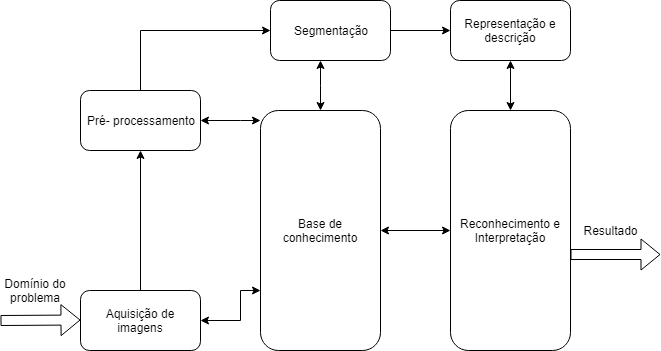
\includegraphics[width=1\textwidth]{./dados/figuras/etapas_processamento_imagens.png}
    \fonte{\citeonline{Gonzalez2000}.}
    \label{fig:etapas_processamento_imagens}
\end{figure}

\par Como observado na \autoref{fig:etapas_processamento_imagens}, para a rotina ser executada é necessário um problema que necessite de um resultado final, assim, com as etapas sendo seguidas corretamente o sucesso da tarefa em questão se torna mais provável. 

\par Sendo assim, o processamento digital de imagens inicia-se a partir da aquisição. Para isto, normalmente aparenta-se necessárias câmeras digitais, porém não é apenas tal dispositivo que é capaz de captar sinais e transformá-los em uma imagem digital, também existem outros sensores de imageamento, basta que este possa captar uma banda do espectro de energia eletromagnética. Após a captura é necessário um dispositivo conhecido como digitalizador, o qual é responsável por converter as informações dos sensores que captaram a informação em uma saída digital.

\par A segunda etapa é o pré-processamento de uma imagem que tem como objetivo principal aumentar as chances de sucesso para as próximas etapas, sendo assim necessário aplicar técnicas como as de isolamento de regiões, remoção de ruídos e outras. De tal forma que o resultado final esperado seja de uma imagem consideravelmente melhor quando comparada com a imagem anterior.

\par Em seguida se encontra a considerada mais difícil etapa do processamento digital de imagens: a segmentação. O uso de algoritmos fracos neste momento pode causar uma falha em todo o processo. Apenas algoritmos adequados podem auxiliar e aumentar a garantia de sucesso ao final. Logo, a segmentação é responsável por decompor a imagem em partes ou objetos, obtendo como resultado \textit{pixels}, conhecidos como \textit{raw pixel data}, o que representa uma área e suas bordas, sendo sempre necessária a conversão dos dados para o uso computacional.

\par Já a etapa de representação e descrição, também conhecida como seleção de características, é responsável por identificar novas características em uma área anteriormente identificada, as quais são referentes a cor, textura e/ou forma.

\par Por fim, na última etapa, reconhecimento e interpretação, se dá a rotulação de um ``objeto'' previamente segmentado, ou seja, a imagem é totalmente ou parcialmente reconhecida. Além disso, para um conjunto de ``objetos'' é concedido um significado, o que se refere a interpretação \cite{Gonzalez2009}.

%% Para futuras melhorias seria interessante fazer uma nova seção sobre os métodos de descrição de imagem e outro de árvore geradora mínima

% Descrição de imagens
% \section{DESCRIÇÃO DE IMAGENS}
% \label{sec:descimg}



% TEXTURA
\subsection{TEXTURA}
\par A textura, elemento importante neste trabalho, pode ser interpretada por diversas óticas, entre elas a popular, pois é de fácil compreensão já que existem em tudo que é visível. Neste sentido, pode-se entender que não é possível estabelecer uma única definição teórica \cite{liberman1997}. 
\par Para \citeonline{haralickTEXTURA}, texturas podem ser determinadas por seu \textit{``layout''}, organização e níveis de cinza. Entretanto, neste trabalho é adotada principalmente a abordagem de \citeonline{Gonzalez2009}, que reafirmam a impossibilidade de definição formal para a propriedade de textura, mas indicam que a rugosidade, suavidade e outros aspectos seriam resultados de descritores como o algoritmo desenvolvido neste projeto, que descreve e classifica texturas em imagens. 

\begin{comment}
\par As abordagens: estatística, estrutural e espectral são as três abordagens mais utilizadas para descrição de texturas em imagens. \cite{Gonzalez2000}
\par Estatística -> suave, aspera, graunular e etc
\par Estruturais -> tratam de arranjos de primitivas de imagem como a descrição da textura baseada em linhas paralelas regularmente espaçadas.
\par Espectrais -> baseiam-se em propriedades do espectro de Fourier, sendo usadas basicamente na detecção de periodicidade global em uma imagem através da identificação de picos de alta-energia no espectro
\par Falar das abordagens: estatísticas, estruturais e espectrais
\end{comment}
%%%%%%%%%%%%%%%%%%%%%%%%%%%%%%%%%%%%%%%%%%%%%%%%%%%%%%%%%%%%%%%%%%%%

% Arvore geradora mínima
\section{ÁRVORE GERADORA MÍNIMA}
\label{sec:arvore}

\par Árvores geradoras mínimas costumam solucionar diversos problemas, um exemplo de sua performance está em projetos de circuitos eletrônicos, pois muitas vezes é necessário fazer a conexão entre pinos de modo que estes estejam eletricamente equivalentes. Tal conexão deve ser feita utilizando o menor custo possível, ou seja, o mínimo de material (fiação). Isto caracteriza um problema que procura encontrar a MST dado um grafo \cite{algoritmos}.

\par Considerando um grafo conexo não dirigido $G$ que pode ser representado por $G = (V, E)$, onde $V$ é o conjunto de todos os vértices e $E$ o conjunto de todas as ligações possíveis entre os vértices do grafo $G$. Todas as arestas formadas por uma conexão de um vértice ao outro, representado por $(u, v) \in E$, devem possuir pesos, ou seja, o custo de um vértice ao outro, que simboliza $w(u, v)$. O que é procurado é uma conexão que esteja contida em $E$ de forma que gere um novo grafo $T$ acíclico e conecte todos os vértices. Dessa maneira, conclui-se que uma árvore geradora mínima é um grafo acíclico que busca percorrer o menor caminho possível e que está contido e gerado a partir de um outro grafo \cite{algoritmos}.

\par Uma representação de um grafo conexo e uma árvore geradora mínima pode ser observada na \autoref{fig:mst}. Todas as arestas pertencem ao grafo, sendo as arestas sombreadas\footnote{Como a aresta que liga os vértices $a$ e $b$} correspondentes à árvore geradora mínima. Também é possível observar que todas as arestas são ponderadas e que o peso total da árvore corresponde a 37. Além disso, esta não é a única MST presente no grafo, pois caso a aresta $(a, b)$ seja trocada pela aresta $(a, h)$, haverá outra MST também com o peso total 37 \cite{algoritmos}.

\begin{figure}[!h]
    \centering
    \caption{Grafo conexo e MST}
    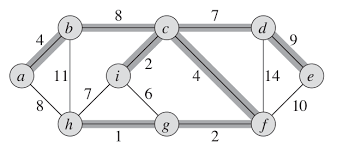
\includegraphics[width=0.7\textwidth]{./dados/figuras/grafo-mst.png}
    \fonte{\citeonline{algoritmos}.}
    \label{fig:mst}
\end{figure}

\par O termo conhecido como ``árvore geradora mínima`` é uma redução da sentença ``árvore geradora de peso mínimo``. Tal explicação se faz necessária, pois existe a possibilidade de que o termo mais comum gere a má interpretação de que o número de arestas de uma árvore geradora foi diminuído, o que não corresponde à verdade.

\subsection{ALGORITMOS}
\label{subsec:algoritmosmst}

\par Existem dois algoritmos principais que buscam resolver o problema da MST, estes são: o algoritmo de Kruskal e o algoritmo de Prim. Ambos são considerados gulosos\footnote{Segundo \citeonline{algoritmos}, os algoritmos gulosos consideram sempre a escolha do momento como a melhor escolha possível, acreditando que esta traga consigo o melhor resultado.}. Apesar de não garantirem resultados considerados excelentes, isto se diverge, ou seja, os algoritmos gulosos podem produzir uma MST dado um determinado grafo.
\par Neste projeto, será utilizado o algoritmo de Prim, pois segundo \citeonline{igraph}, este é implementado na biblioteca \textit{igraph} para o método que gera uma MST, dado um grafo e seus pesos. Maiores detalhes, sobre esta e outras bibliotecas utilizadas podem ser observados na \autoref{sec:tecnologiasferramentas}.

% Uso de Grafos em descrição de imagens
\section{USO DE GRAFOS EM DESCRIÇÃO DE IMAGENS}
\label{sec:usografosdescimg}

\par A partir de pesquisas sobre o estado da arte desta área foi possível concluir que, no momento atual de desenvolvimento deste trabalho, não existem publicações sobre a aplicação de MST para a descrição de texturas em imagens, sendo os únicos encontrados, trabalhos que utilizam árvores geradoras mínimas para a segmentação, registro, detecção de imagens ou outros.

\par Sendo assim, apesar de poucos trabalhos buscarem a utilização de outros tipos de algoritmos com grafos e árvores para descrição de imagens, é possível observar que nestes há uma melhoria considerável, o que estimula o desenvolvimento de novos métodos de pesquisa em vários campos de processamento de imagens e computação visual, assim como proposto por este trabalho.

\subsection{\textit{SHORTEST PATHS} EM DESCRIÇÃO DE IMAGENS}
\label{subsec:trabalho-jarbas}

\par O estudo que mais se assemelha com a proposta deste trabalho é o de \citeonline{jarbas-color-texture}, que tem como título: \textit{Color Texture Classification Using Shortest Paths in Graphs}. Apesar de utilizarem o algoritmo de \textit{shortest paths}, caminho mais curto, se aproximam pelo estudo de textura da imagem, a ligação entre os vértices e a forma como a imagem é ``tranformada'' em grafo.

\par Neste trabalho, o algoritmo desenvolvido obteve resultados significativos e potentes na extração de informações presentes na textura das imagens analisadas, sobressaindo até mesmo algoritmos bem estabelecidos atualmente. Desta forma, pode-se concluir que a utilização de grafos para descrição de texturas em imagens se mostra como uma boa oportunidade de campo novo a ser explorado, e que pode auxiliar no aumento da acurácia e confiança em sistemas de computação visual.

% Proposta
% PROPOSTA------------------------------------------------------------------

\chapter{DESENVOLVIMENTO}
\label{chap:proposta}

\par Este trabalho tem como proposta a construção de um algoritmo para a identificação e descrição de texturas de imagens através da aplicação de árvores geradoras mínimas. Sendo assim, neste capítulo serão esclarecidas as ações tomadas nas diferentes etapas do projeto e as ferramentas utilizadas para a sua execução.

\section{MÉTODO}
\label{sec:metodo}

\par O método de desenvolvimento utilizado possui 6 etapas principais, as quais estão listadas a seguir e se encontram em ordem de execução:

\begin{enumerate}
    \item Selecionar uma imagem;
    \item A partir da imagem, convertê-la em um grafo sem arestas, no qual cada pixel representa um vértice e armazena o seu valor;
    \item Ligar todos os \textit{pixels} com seus vizinhos, caracterizando vizinhança 8, ou 4 caso o \textit{pixel} esteja na borda;
    \item Atribuir valores (pesos) a cada aresta do grafo formado. Este valor corresponde ao módulo da diferença entre os valores do pixel em \textit{8-bits}, ou seja, valores entre 0 e 255;
    \item Encontrar uma árvore geradora mínima do grafo;
    \item Extrair um vetor de características a partir dos valores obtidos em cada aresta da MST, tal vetor é formado pela: média simples, desvio padrão, grau de assimetria, curtose e entropia.
    % \item Analisar resultado obtido;
    % \item Repetir os passos anteriores com um \textit{dataset} de várias imagens;
    % \item Comparar o algoritmo realizado com outros algoritmos presentes na literatura;
    % \item Analisar resultados obtidos e fazer as devidas modificações e aprimoramentos.
\end{enumerate}

\par A \autoref{fig:metodo} ilustra o método descrito acima, com o intuito de facilitar a compreensão e retratar de forma mais objetiva e concisa. Em seguida, cada etapa será descrita de forma mais detalhada.

\begin{figure}[h]
    \centering
    \caption{Diagrama de etapas do método desenvolvido}
    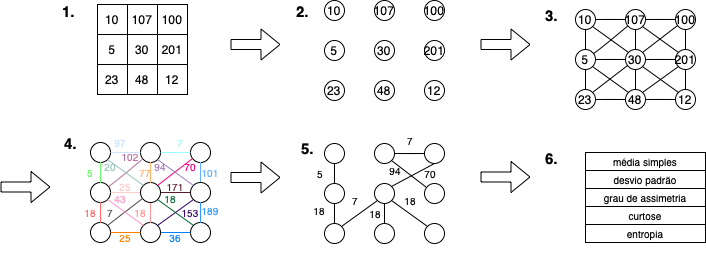
\includegraphics[width=1\textwidth]{./dados/figuras/metodo.png}
    \fonte{Autoria Própria}
    \label{fig:metodo}
\end{figure}

\par Na etapa 1, é obtida a imagem, onde cada \textit{pixel} contém o seu valor. Na segunda etapa, a imagem é convertida para um grafo, ainda sem arestas, onde cada vértice contém o valor do \textit{pixel}. Já na etapa 3, são feitas todas as ligações possíveis de um vértice com o seus vizinhos, considerando vizinhança-8 ou vizinhança-4, caso o vértice esteja localizado na borda. Na quarta etapa, as arestas são ponderadas, ou seja, são atribuídos valores a estas, sendo esse valor correspondente ao módulo da diferença entre os dois vértices. Na penúltima etapa, é formada a árvore geradora mínima. Por fim, na etapa 6, a partir dos valores das arestas da MST obtida, é formado um vetor por cinco características: média simples, desvio padrão, grau de assimetria, curtose e entropia.
\begin{comment}
\par Por fim, vale ressaltar que este processo poderá ser realizado diversas vezes em uma mesma imagem, de forma a serem obtidas diferentes MST. Isto será possível, de modo que, algumas arestas e vértices serão eliminados propositalmente após a quarta fase, deste modo o que caracterizará a eliminação destes será um valor específico, maior ou menor que um valor empírico obtido durante os experimentos. Além disto, o valor será padronizado com estimativas de média e desvio padrão, antes da sexta etapa, de forma que um mesmo grafo que possua diversas MST não será necessário analisar-se todas as possibilidades, de forma a garantir um vetor de características padronizado.
\end{comment}

%% Parte escrita sobre o cascata-----------------------------------------------
\begin{comment}
\par Para a aplicação do trabalho, será utilizado o modelo cascata como processo de software, como pode ser observado na figura \ref{fig:modelo_cascata}, que representa tal modelo segundo \citeonline{Sommerville2011}. 

\begin{figure}[!h]
    \centering
    \caption{O modelo cascata}
    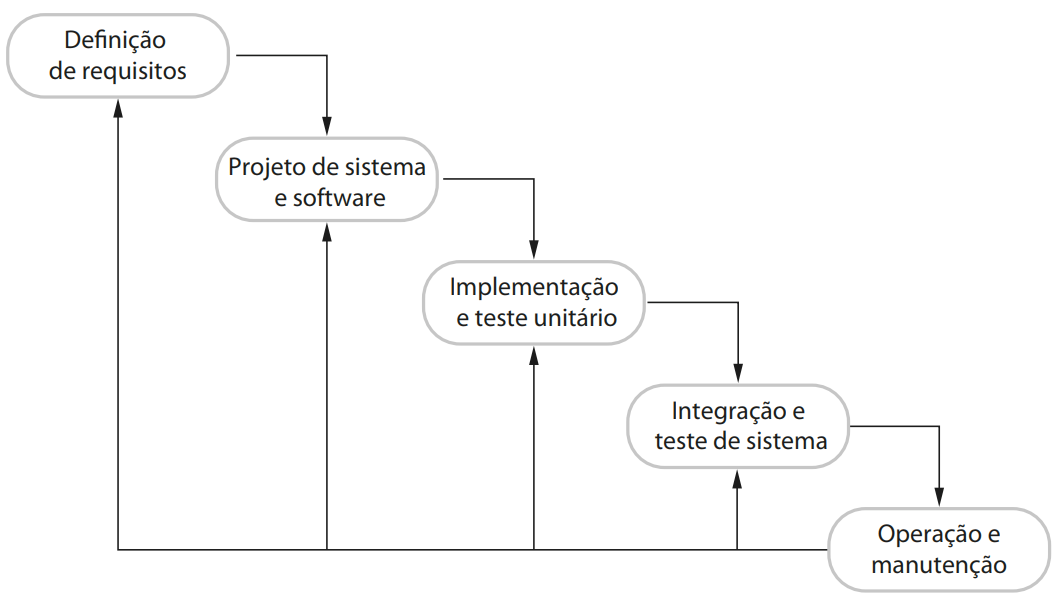
\includegraphics[width=1\textwidth]{./dados/figuras/modelo_cascata.png}
    \fonte{\citeonline{Sommerville2011}}
    \label{fig:modelo_cascata}
\end{figure}
\par Abaixo estão descritas cada fase do processo, que devem ser previamente planejadas e quais seus objetivos a serem cumpridos. Foi utilizado como base o trabalho de \citeonline{Sommerville2011} onde o autor define cada fase e as detalha.
\par Na etapa de comunicação, também conhecida como definição de requisitos, é onde serão elicitados os requisitos funcionais e não funcionais, resultando em uma melhor descrição do programa.
\par No projeto de sistema de software será realizado um planejamento, através do desenvolvimento do cronograma geral. O primeiro cronograma desenvolvido para o projeto pode ser visualizado no capítulo \ref{chap:cronograma} desse trabalho. Também haverá modelagem, a qual vai abordar a construção de alguns diagramas UML, tendo como objetivo maior a validação dos requisitos levantados anteriormente. Além de uma análise da estrutura geral do projeto com diagramas de classes e sequência.
\par A fase de implementação e teste unitário, se refere à construção de pequenos módulos e testes dos mesmos, utilizando das ferramentas e tecnologias anteriormente descritas e tendo como foco os requisitos.
\par Já a integração e teste de sistema é um complemento da fase anterior, onde todos os módulos implementados deverão ser integrados de forma a compor um único programa, o qual deve ser testado.
\par Por fim, a última etapa expõe a entrega final, quando o algoritmo, o documento e a validação devem se encontrar finalizados. No entanto, essa fase também diz a respeito de um \textit{feedback} do orientador, onde serão corrigidos e aprimorados certos módulos.
\end{comment}
%% Fim Parte escrita sobre o cascata-----------------------------------------------

\section{DESENVOLVIMENTO DO ALGORITMO}
\label{sec:desenvolvimentoalgoritmo}

\par A partir do uso das ferramentas, \autoref{sec:tecnologiasferramentas}, da busca pelo alcance dos objetivos descritos na \autoref{subsec:objgerais} e da aplicação do método elaborado, \autoref{sec:metodo}, foi possível desenvolver o algoritmo que será descrito nesta subseção.

\par O algoritmo em si deverá ligar todos os \textit{pixels} com seus vizinhos\footnote{Vizinhança-8 ou vizinhança-4, caso este seja um \textit{pixel} que esteja localizado na borda da imagem.}, o que irá formar um grafo. Cada aresta deste grafo receberá um peso, sendo representado pelo módulo da diferença do \textit{pixel} com o seu vizinho. A partir do grafo formado, utilizando a biblioteca \textit{igraph}, será gerado um segundo grafo correspondente a árvore geradora mínima\footnote{Vale ressaltar que tal MST formada a partir do primeiro grafo, também está contida neste.} a partir dos pesos das arestas.

\subsection{PRIMITIVAS}
\label{subsec:primitivas}

\par O algoritmo desenvolvido busca, a partir de uma imagem digital, descrever e identificar a sua textura, através de MST. Para que fosse possível alcançar o seu objetivo, foram definidas algumas primitivas consideradas para o desenvolvimento, as mesmas estão disponíveis em seguida:

\begin{itemize}
    \item Deve-se utilizar as ferramentas e tecnologias descritas na  \autoref{sec:tecnologiasferramentas};
    \item O algoritmo deve seguir o método presente na \autoref{sec:metodo};
    \item Os pesos das arestas do grafo devem ser um parâmetro de fácil modificação. Isto se torna importante pois possibilita a troca do critério que forma o peso das arestas, o que pode ser usado em outros testes resultando na melhoria do algoritmo e consequentemente em sua manutenção;
    \item Devem ser consideradas somente imagens em formato \textit{png}, imagens em outros formatos podem ser convertidas mantendo aproximadamente o tamanho em \textit{bytes} atual;
    \item Precisam ser consideradas apenas imagens em escala de cinza, utilizando da biblioteca \textit{Scikit-Image} \cite{ScikitImage} para converter imagens que não estiverem em tal escala;
    \item Por fim, devem ser consideradas imagens em \textit{8-bits}, ou seja, que apresentem um valor entre 0 e 255, utilizando também a biblioteca \textit{Scikit-Image} \cite{ScikitImage} para converter imagens quando necessário.
\end{itemize}

\section{TECNOLOGIAS E FERRAMENTAS}
\label{sec:tecnologiasferramentas}

\par Atualmente existem várias ferramentas que podem auxiliar o processamento digital de imagens, sendo uma dessas a \textit{Open Source Computer Vision Library} (\textit{OpenCV}).
A biblioteca \textit{OpenCV} é produzida em C++ e atualmente está disponível para uso para as linguagens de programação: \textit{python}, \textit{java}, linguagem C e C++ \cite{opencv_library}.

\par Tal biblioteca, aberta à comunidade, possui uma estrutura modular, de forma que alguns de seus módulos sejam: processamento de imagens, análise de vídeo, calibração de câmera e reconstrução em 3D, funcionalidades de \textit{framework} 2D, detecção de objetos, \textit{Graphical User Interface} (GUI) de alto nível, entrada e saída de vídeo, entre outros \cite{opencv_library}.

\par No entanto, este projeto será desenvolvido utilizando a biblioteca \textit{Scikit-Image}, a qual também é \textit{open-source} e está em constante atualização, como é possível observar em seu \textit{github}. Esta biblioteca é escrita em \textit{python} e também é utilizada por programas escritos em \textit{python}.

\par A \textit{Scikit-Image} possui várias funções que podem ser facilmente utilizadas, fornecendo rotinas versáteis e intuitivas de processamento digital de imagens, provendo sub-módulos dedicados a: cor, desenho, exposição, análise de texturas e bordas, grafos, entrada e saída, entre tantos outros que indiscutivelmente podem auxiliar a muitos na construção de um \textit{software} destinado a processamento de imagens  \cite{ScikitImage}.

\par A escolha de tal biblioteca foi dada principalmente devido as suas funcionalidades que estão em constante atualização, por ser feita nativamente em \textit{python}, seu uso ser intuitivo e vários outros aspectos que a tornam mais interessante que a \textit{OpenCV} para este projeto.

\par Como linguagem de programação, será adotada a linguagem \textit{python}, pois possui consigo várias vantagens, que podem ser observadas facilmente em seu \textit{website} e \textit{github}, tais como: a vasta coleção de bibliotecas, sendo várias de cunho científico, a possibilidade da escrita de códigos legíveis e sua comunidade presenta na evolução da linguagem, por ser \textit{open-source}.

\par Por fim, será utilizada a biblioteca \textit{igraph}, que irá auxiliar a construir os grafos para uma determinada imagem e também encontrar a árvore geradora mínima \cite{igraph}. Além da biblioteca \textit{scikit-learn} a qual será utilizada durante as validações para testar o algoritmo e compará-lo a outros já existentes. \cite{scikit-learn}.

\section{VALIDAÇÕES}
\label{sec:validacoes}

\par Assim que o algoritmo tenha atendido todas as primitivas e cumprido com o esperado, será necessário comprovar a sua eficácia. Para isto, o algoritmo será comparado com outros métodos de descrição de imagens, mais especificamente de texturas, já presentes na literatura, sendo estes: Gabor \cite{gaborZhang2000content}, Haralick \cite{haralick1973textural}, \textit{local binary patterns} (LBP) \cite{lbp-guo2010rotation} e Tamura \cite{tamura1978textural}.

\par De modo a comparar os extratores, serão realizados alguns testes com diferentes algoritmos de aprendizado supervisionado, como: \textit{decision tree}, k-nearest neighbors (KNN), \textit{linear support vector classification} (\textit{Linear} SVC) e \textit{c-support vector classification} (SVC).

\par Para o algoritmo de aprendizado supervisionado, deve-se manter a semente com um valor igual a 5 (cinco), garantindo que, ao ser executado com as mesmas condições, o algoritmo sempre desempenhe os mesmos resultados. Além disso, deve-se separar o \textit{dataset} em 20\% teste e 80\% treino, ser capaz de ler arquivos em formato \textit{attribute-relation file format} (ARFF) e \textit{comma-separated values} (CSV).

\par Dessa forma, os resultados devem ser salvos para consulta posterior e apresentar: acurácia, precisão, \textit{recall}, \textit{f-score}, matriz de confusão e relatório de classificação por classes. Assim, as acurácias obtidas pelos extratores serão comparadas quando testados com diferentes algoritmos de aprendizado supervisionado, além da análise da matriz de confusão. Por fim, será calculado o tempo de execução dos extratores.

\begin{comment}
\par Além disso, serão utilizados algoritmos de classificação supervisionada para apresentar taxas de acerto, eficácia e a eficiência.

\par Como variável de comparação será primeiramente utilizada a capacidade do código de descrever a textura de uma imagem, quando comparado a outros algoritmos bem aceitos pela comunidade científica, os quais também foram citados anteriormente. Dessa forma, serão analisados entre os algoritmos, quais são capazes de oferecer o melhor resultado final, ou seja, a partir de uma imagem, sejam capazes de apresentar dados da textura e suas características.

\par Com o uso da biblioteca \textit{scikit-learn}, é esperado como resultado final uma taxa de acurácia e uma análise da matriz de confusão da comparação entre os procedimentos.

\par Além disso, também será comparada, porém em segunda instância, o custo computacional dos algoritmos. Sendo tomado vez o tempo de execução e vez o uso de memória primária e processamento. Esta validação será considerada principal caso a outra validação mostre que o algoritmo não obteve um resultado satisfatório, porém pode ser levado em consideração caso este se mostre mais eficiente que outros nestes aspectos.

\par Por fim, vale ressaltar que serão utilizadas as seguintes bases de dados: Vison Texture Database (VisTex) \cite{vistex} e a USPTex \cite{usptex}.
\end{comment}

\subsection{DATASETS}
\label{subsec:datasets}

\par Para testar o algoritmo são necessárias imagens, para isto alguns \textit{datasets} fornecem uma quantidade vasta de imagens que são dividas em grupos. Dessa forma, foram escolhidos quatro \textit{datasets} com foco para testar a característica de textura de algoritmos de extração de características.

\subsubsection{USC-SIPI TEXTURES}
\label{subsubsec:usc-spi}

\par O USC-SIPI \textit{Textures} \cite{weber1997usc} é um \textit{dataset} composto por um conjunto de imagens, entre essas algumas extraídas do \textit{dataset} Brodatz \cite{brodatz1966textures}, o qual segundo \citeonline{fekri2019new}, é formado através de fotografias digitalizadas para diversos propósitos, o que o torna um dos mais populares.
\par O \textit{dataset} possui somente imagens monocromáticas, \textit{8-bits}, sendo a resolução de 130 destas 512x512 \textit{pixels} e 25 de 1024x1024 \textit{pixels}, totalizando 155 imagens. No entanto, para a validação foi utilizado o \textit{dataset} com imagens rotacionadas em sete graus diferentes: 0, 30, 60, 90, 120, 150 e 200 graus, totalizando 91 imagens de 512x512 \textit{pixels}. Este \textit{dataset} possui um total de 13 classes, alguns exemplos de imagens podem ser observados na \autoref{fig:usc-sipi} \cite{weber1997usc}. Por fim, suas classes são: \textit{Bark}, \textit{Brick}, \textit{Bubbles}, \textit{Grass}, \textit{Leather}, \textit{Pigskin}, \textit{Raffia}, \textit{Sand}, \textit{Straw},
\textit{Water}, \textit{Weave}, \textit{Wood}, \textit{Wool} \cite{weber1997usc}.

\begin{figure}[!h]
    \centering
    \caption{Exemplos de imagens disponíveis no \textit{dataset} USC-SIPI \textit{Textures}.}
    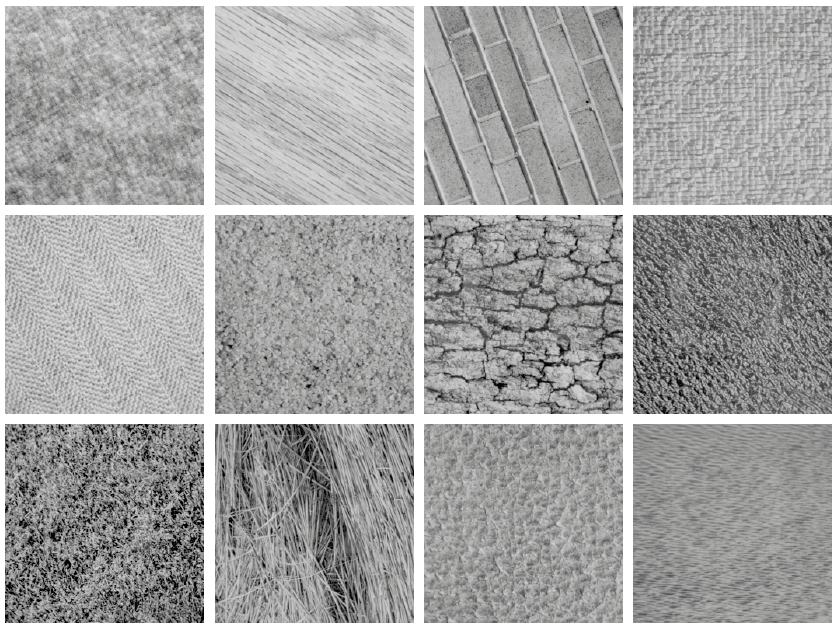
\includegraphics[width=0.7\textwidth]{./dados/figuras/usc-sipi.png}
    \fonte{\citeonline{weber1997usc}}
    \label{fig:usc-sipi}
\end{figure}

% KYBERG
\subsubsection{KYLBERG}
\label{subsubsec:kylberg}

\par Segundo \citeonline{Kylberg2011c}, seu \textit{dataset} possui 28 classes, sendo que cada uma possui 160 imagens em resolução 576x576 \textit{pixels}, \textit{8-bits} e formato PNG. Além de todas imagens serem normalizadas com desvio padrão correspondendo a 40 e um valor médio de 127. A \autoref{fig:kylberg} apresenta algumas imagens pertencentes a este \textit{dataset}.

\begin{figure}[!h]
    \centering
    \caption{Exemplos de imagens disponíveis no \textit{dataset} Kylberg.}
    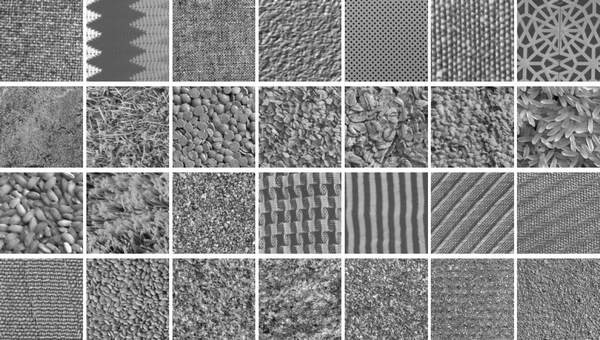
\includegraphics[width=0.7\textwidth]{./dados/figuras/kylberg.jpg}
    \fonte{\citeonline{Kylberg2011c}}
    \label{fig:kylberg}
\end{figure}


\subsubsection{USPTEX}
\label{subsubsec:usptex}

\par Este \textit{dataset} possui um total de 2.292 imagens, dividas em 191 classes, todas com resolução de 128x128 \textit{pixels}, apesar das imagens originais estarem em 512x512 \textit{pixels}. Estas possuem texturas com cores naturais adquiridas sob uma fonte de luz fixa desconhecida, alguns exemplos destas estão disponibilizados na \autoref{fig:usptex} \cite{usptex}.

\begin{figure}[!h]
    \centering
    \caption{Exemplos de imagens disponíveis no USPtex.}
    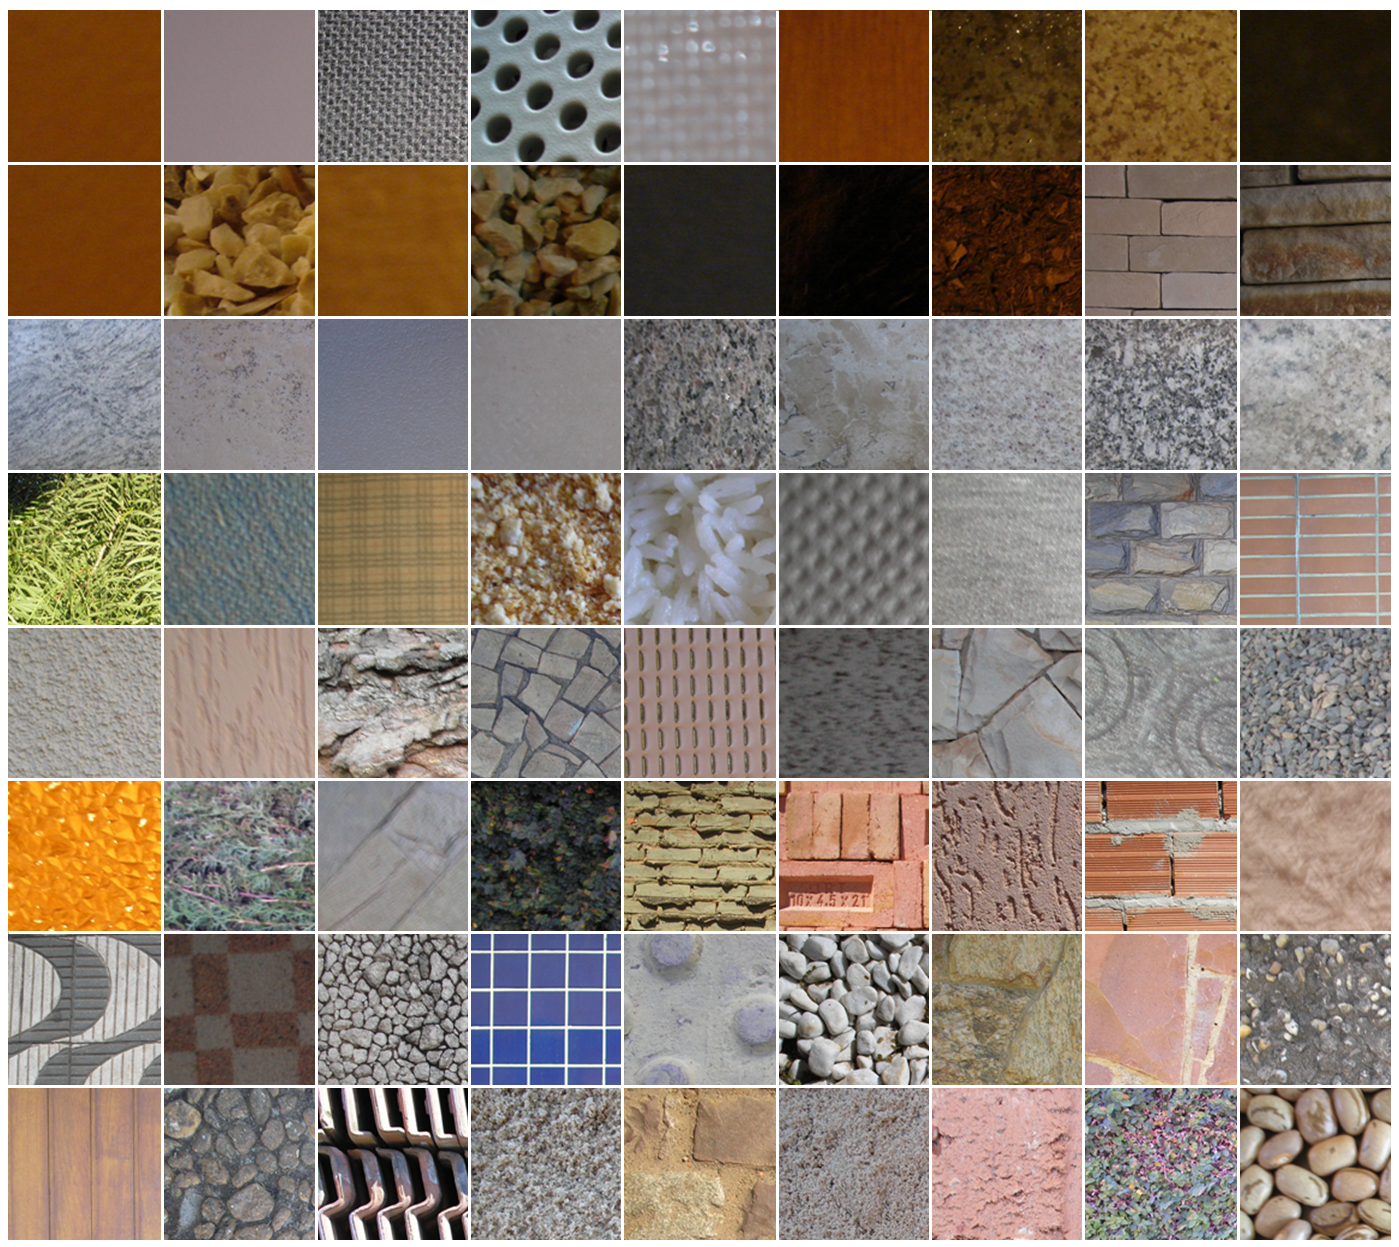
\includegraphics[width=0.7\textwidth]{./dados/figuras/USPtex.png}
    \fonte{\citeonline{usptex}.}
    \label{fig:usptex}
\end{figure}

\subsubsection{VISTEX}
\label{subsubsec:vistex}

\par O \textit{Vision Texture} (VisTex), é um \textit{dataset} que provem uma quantia vasta de texturas de alta qualidade para aplicação em contextos de visão computacional. Dessa forma, as imagens retratam o mundo real e oferecem texturas tanto tradicionais quanto não tão tradicionais \cite{vistex}. Estas imagens são coloridas e possuem uma resolução de 128x128 \textit{pixels} e um total de 40 classes \cite{fekri2019new}. Para os testes foram consideradas 19 classes, totalizando 167 imagens. A \autoref{fig:vistex} expõe algumas exemplos deste \textit{dataset} utilizados nas validações.

\begin{figure}[!h]
    \centering
    \caption{Exemplos de imagens disponíveis no VisTex.}
    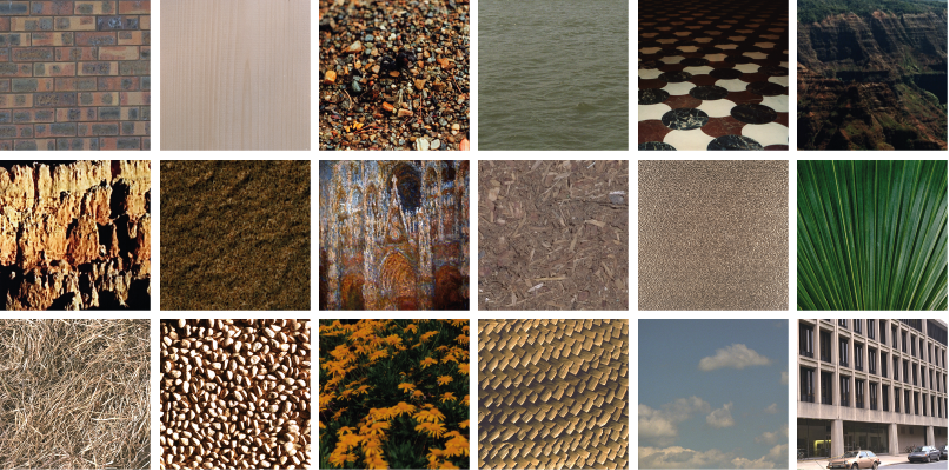
\includegraphics[width=0.7\textwidth]{./dados/figuras/vistex.png}
    \fonte{\citeonline{vistex}}
    \label{fig:vistex}
\end{figure}

\begin{comment} 
\section{CRONOGRAMA}
\label{sec:cronograma}

\par Este capítulo tem como objetivo apresentar um cronograma para o futuro deste projeto. As fases, bem como suas atividades estão listadas logo em seguida e podem ser melhor observadas por meio da \autoref{tab:cronograma} e também através da \autoref{tab:cronograma-fases} as quais fazem uma relação entre atividades, fases e datas.

Vale ressaltar que as tabelas apresentam um mês e logo abaixo o número 1 e 2, o número 1 faz referência à primeira metade do mês e o número 2 à segunda metade\footnote{Exemplo: Dado o mês de novembro, o número 1 faz referência do dia 1 ao 15, já o número 2 faz referência do dia 16 ao 30.}.


\begin{enumerate}
    \item Correções
        \begin{enumerate}
            \item[1.1] Fazer as devidas correções neste documento, conforme detalhes apresentados pela banca e pelo orientador;
            \item[1.2] Verificar e validar correções.
        \end{enumerate}

    \item Preparação
        \begin{enumerate}
            \item[2.1] Definir premissas;
            \item[2.2] Definir módulos;
            \item[2.3] Verificar e validar;
            \item[2.4] Documentar e escrever sobre esta fase.
        \end{enumerate}

    \item Implementação
        \begin{enumerate}
            \item[3.1] Aprofundar conhecimentos em linguagem \textit{python};
            \item[3.2] Estudar novamente a documentação das bibliotecas e demais ferramentas, focando nos métodos que serão utilizados;
            \item[3.3] Iniciar a programação módulo $n$;
            \item[3.4] Testar o módulo $n$;
            \item[3.5] Documentar e escrever sobre esta fase.
        \end{enumerate}
        
    \item Integração
        \begin{enumerate}
            \item[4.1] Integrar os módulos da fase anterior;
            \item[4.2] Testar a integração;
            \item[4.3] Preparar o teste para a validação do algoritmo;
            \item[4.4] Testar o algoritmo;
            \item[4.5] Documentar e escrever sobre esta fase.
        \end{enumerate}
        
    \item Testes e comparações
        \begin{enumerate}
            \item[5.1] Estudar outros algoritmos de descrição de imagens;
            \item[5.2] Preparar testes entre o algoritmo obtido na fase anterior com os presentes na literatura;
            \item[5.3] Realizar testes;
            \item[5.4] Analisar resultados;
            \item[5.5] Verificar e validar;
            \item[5.6] Documentar e escrever sobre esta fase.
        \end{enumerate}
    
    \item Operação e manutenção
        \begin{enumerate}
            \item[6.1] Observar os resultados da etapa anterior e fazer as devidas modificações para a melhor eficiência do algoritmo;
            \item[6.2] Documentar e escrever sobre esta fase.
        \end{enumerate}
        
    \item Documentação
        \begin{enumerate}
            \item[7.1] Finalizar o documento referente ao Trabalho de Conclusão de Curso 2, utilizando da documentação das fases anteriores, além do documento produzido para o Trabalho de Conclusão de Curso 1;
            \item[7.2] Preparar apresentação.
        \end{enumerate}
        
\end{enumerate}

% Please add the following required packages to your document preamble:
% \usepackage[table,xcdraw]{xcolor}
% If you use beamer only pass "xcolor=table" option, i.e. \documentclass[xcolor=table]{beamer}
\begin{table}[H]
\centering
\caption{Cronograma do projeto por atividades.}
\label{tab:cronograma}
\resizebox{\textwidth}{!}{
\begin{tabular}{|l|l|l|l|l|l|l|l|l|l|l|l|l|l|l|l|l|}
\hline
\multicolumn{17}{|c|}{Cronograma}                                                                                                                                                                                                                                                                                                                                                                                                                                                                                                                     \\ \hline
Ano       & \multicolumn{4}{c|}{2019}                                                                                                        & \multicolumn{12}{c|}{2020}                                                                                                                                                                                                                                                                                                                                                                             \\ \hline
Mês       & \multicolumn{2}{c|}{Novembro}                                              & \multicolumn{2}{c|}{Dezembro}                       & \multicolumn{2}{c|}{Janeiro}                        & \multicolumn{2}{c|}{Fevereiro}                      & \multicolumn{2}{c|}{Março}                                                                        & \multicolumn{2}{c|}{Abril}                                                 & \multicolumn{2}{c|}{Maio}                           & \multicolumn{2}{c|}{Junho}                          \\ \hline
Atividade & \multicolumn{1}{c|}{1}   & \multicolumn{1}{c|}{2}                          & \multicolumn{1}{c|}{1}   & \multicolumn{1}{c|}{2}   & \multicolumn{1}{c|}{1}   & \multicolumn{1}{c|}{2}   & \multicolumn{1}{c|}{1}   & \multicolumn{1}{c|}{2}   & \multicolumn{1}{c|}{1}                          & \multicolumn{1}{c|}{2}                          & \multicolumn{1}{c|}{1}                          & \multicolumn{1}{c|}{2}   & \multicolumn{1}{c|}{1}   & \multicolumn{1}{c|}{2}   & \multicolumn{1}{c|}{1}   & \multicolumn{1}{c|}{2}   \\ \hline
1.1       & \cellcolor[HTML]{000000} &                                                 &                          &                          &                          &                          &                          &                          &                                                 &                                                 &                                                 &                          &                          &                          &                          &                          \\ \hline
1.2       & \cellcolor[HTML]{000000} &                                                 &                          &                          &                          &                          &                          &                          &                                                 &                                                 &                                                 &                          &                          &                          &                          &                          \\ \hline
2.1       &                          & \cellcolor[HTML]{000000}{\color[HTML]{000000} } &                          &                          &                          &                          &                          &                          &                                                 &                                                 &                                                 &                          &                          &                          &                          &                          \\ \hline
2.2       &                          & \cellcolor[HTML]{000000}                        &                          &                          &                          &                          &                          &                          &                                                 &                                                 &                                                 &                          &                          &                          &                          &                          \\ \hline
2.3       &                          & \cellcolor[HTML]{000000}                        &                          &                          &                          &                          &                          &                          &                                                 &                                                 &                                                 &                          &                          &                          &                          &                          \\ \hline
2.4       &                          & \cellcolor[HTML]{000000}                        &                          &                          &                          &                          &                          &                          &                                                 &                                                 &                                                 &                          &                          &                          &                          &                          \\ \hline
3.1       &                          &                                                 & \cellcolor[HTML]{000000} &                          &                          &                          &                          &                          &                                                 &                                                 &                                                 &                          &                          &                          &                          &                          \\ \hline
3.2       &                          &                                                 & \cellcolor[HTML]{000000} &                          &                          &                          &                          &                          &                                                 &                                                 &                                                 &                          &                          &                          &                          &                          \\ \hline
3.3       &                          &                                                 & \cellcolor[HTML]{000000} & \cellcolor[HTML]{000000} & \cellcolor[HTML]{000000} & \cellcolor[HTML]{000000} &                          &                          &                                                 &                                                 &                                                 &                          &                          &                          &                          &                          \\ \hline
3.4       &                          &                                                 & \cellcolor[HTML]{000000} & \cellcolor[HTML]{000000} & \cellcolor[HTML]{000000} & \cellcolor[HTML]{000000} &                          &                          &                                                 &                                                 &                                                 &                          &                          &                          &                          &                          \\ \hline
3.5       &                          &                                                 &                          &                          &                          & \cellcolor[HTML]{000000} &                          &                          &                                                 &                                                 &                                                 &                          &                          &                          &                          &                          \\ \hline
4.1       &                          &                                                 &                          &                          &                          &                          & \cellcolor[HTML]{000000} &                          &                                                 &                                                 &                                                 &                          &                          &                          &                          &                          \\ \hline
4.2       &                          &                                                 &                          &                          &                          &                          & \cellcolor[HTML]{000000} &                          &                                                 &                                                 &                                                 &                          &                          &                          &                          &                          \\ \hline
4.3       &                          &                                                 &                          &                          &                          &                          & \cellcolor[HTML]{000000} &                          &                                                 &                                                 &                                                 &                          &                          &                          &                          &                          \\ \hline
4.4       &                          &                                                 &                          &                          &                          &                          & \cellcolor[HTML]{000000} &                          &                                                 &                                                 &                                                 &                          &                          &                          &                          &                          \\ \hline
4.5       &                          &                                                 &                          &                          &                          &                          & \cellcolor[HTML]{000000} &                          &                                                 &                                                 &                                                 &                          &                          &                          &                          &                          \\ \hline
5.1       &                          &                                                 &                          &                          &                          &                          &                          & \cellcolor[HTML]{000000} &                                                 &                                                 &                                                 &                          &                          &                          &                          &                          \\ \hline
5.2       &                          &                                                 &                          &                          &                          &                          &                          & \cellcolor[HTML]{000000} &                                                 &                                                 &                                                 &                          &                          &                          &                          &                          \\ \hline
5.3       &                          &                                                 &                          &                          &                          &                          &                          &                          & \cellcolor[HTML]{000000}{\color[HTML]{000000} } &                                                 &                                                 &                          &                          &                          &                          &                          \\ \hline
5.4       &                          &                                                 &                          &                          &                          &                          &                          &                          & \cellcolor[HTML]{000000}{\color[HTML]{000000} } &                                                 &                                                 &                          &                          &                          &                          &                          \\ \hline
5.5       &                          &                                                 &                          &                          &                          &                          &                          &                          & \cellcolor[HTML]{000000}{\color[HTML]{000000} } &                                                 &                                                 &                          &                          &                          &                          &                          \\ \hline
5.6       &                          &                                                 &                          &                          &                          &                          &                          &                          & \cellcolor[HTML]{000000}{\color[HTML]{000000} } &                                                 &                                                 &                          &                          &                          &                          &                          \\ \hline
6.1       &                          &                                                 &                          &                          &                          &                          &                          &                          &                                                 & \cellcolor[HTML]{000000}{\color[HTML]{000000} } & \cellcolor[HTML]{000000}{\color[HTML]{000000} } & \cellcolor[HTML]{000000} & \cellcolor[HTML]{000000} &                          &                          &                          \\ \hline
6.2       &                          &                                                 &                          &                          &                          &                          &                          &                          &                                                 & \cellcolor[HTML]{000000}{\color[HTML]{000000} } & \cellcolor[HTML]{000000}{\color[HTML]{000000} } & \cellcolor[HTML]{000000} & \cellcolor[HTML]{000000} &                          &                          &                          \\ \hline
7.1       &                          &                                                 &                          &                          &                          &                          &                          &                          &                                                 &                                                 &                                                 & \cellcolor[HTML]{000000} & \cellcolor[HTML]{000000} & \cellcolor[HTML]{000000} & \cellcolor[HTML]{000000} &                          \\ \hline
7.2       &                          &                                                 &                          &                          &                          &                          &                          &                          &                                                 &                                                 &                                                 &                          &                          & \cellcolor[HTML]{000000} & \cellcolor[HTML]{000000} & \cellcolor[HTML]{000000} \\ \hline
\end{tabular}
}
\end{table}

Uma visão mais resumida e menos detalhada pode ser vista na \autoref{tab:cronograma-fases}, estando esta organizada através das fases do projeto, definidas no início desta \autoref{sec:cronograma}.

% Please add the following required packages to your document preamble:
% \usepackage[table,xcdraw]{xcolor}
% If you use beamer only pass "xcolor=table" option, i.e. \documentclass[xcolor=table]{beamer}
\begin{table}[H]
\centering
\caption{Cronograma do projeto por fases.}
\label{tab:cronograma-fases}
\resizebox{\textwidth}{!}{
\begin{tabular}{|l|l|l|l|l|l|l|l|l|l|l|l|l|l|l|l|l|}
\hline
\multicolumn{17}{|c|}{Cronograma}                                                                                                                                                                                                                                                                                                                                                                                                                    \\ \hline
Ano  & \multicolumn{4}{c|}{2019}                                                                                 & \multicolumn{12}{c|}{2020}                                                                                                                                                                                                                                                                                                        \\ \hline
Mês  & \multicolumn{2}{c|}{Novembro}                       & \multicolumn{2}{c|}{Dezembro}                       & \multicolumn{2}{c|}{Janeiro}                        & \multicolumn{2}{c|}{Fevereiro}                      & \multicolumn{2}{c|}{Março}                          & \multicolumn{2}{c|}{Abril}                          & \multicolumn{2}{c|}{Maio}                           & \multicolumn{2}{c|}{Junho}                          \\ \hline
Fase & \multicolumn{1}{c|}{1}   & \multicolumn{1}{c|}{2}   & \multicolumn{1}{c|}{1}   & \multicolumn{1}{c|}{2}   & \multicolumn{1}{c|}{1}   & \multicolumn{1}{c|}{2}   & \multicolumn{1}{c|}{1}   & \multicolumn{1}{c|}{2}   & \multicolumn{1}{c|}{1}   & \multicolumn{1}{c|}{2}   & \multicolumn{1}{c|}{1}   & \multicolumn{1}{c|}{2}   & \multicolumn{1}{c|}{1}   & \multicolumn{1}{c|}{2}   & \multicolumn{1}{c|}{1}   & \multicolumn{1}{c|}{2}   \\ \hline
1    & \cellcolor[HTML]{000000} &                          &                          &                          &                          &                          &                          &                          &                          &                          &                          &                          &                          &                          &                          &                          \\ \hline
2    &                          & \cellcolor[HTML]{000000} &                          &                          &                          &                          &                          &                          &                          &                          &                          &                          &                          &                          &                          &                          \\ \hline
3    &                          &                          & \cellcolor[HTML]{000000} & \cellcolor[HTML]{000000} & \cellcolor[HTML]{000000} & \cellcolor[HTML]{000000} &                          &                          &                          &                          &                          &                          &                          &                          &                          &                          \\ \hline
4    &                          &                          &                          &                          &                          &                          & \cellcolor[HTML]{000000} &                          &                          &                          &                          &                          &                          &                          &                          &                          \\ \hline
5    &                          &                          &                          &                          &                          &                          &                          & \cellcolor[HTML]{000000} & \cellcolor[HTML]{000000} &                          &                          &                          &                          &                          &                          &                          \\ \hline
6    &                          &                          &                          &                          &                          &                          &                          &                          &                          & \cellcolor[HTML]{000000} & \cellcolor[HTML]{000000} & \cellcolor[HTML]{000000} & \cellcolor[HTML]{000000} &                          &                          &                          \\ \hline
7    &                          &                          &                          &                          &                          &                          &                          &                          &                          &                          &                          & \cellcolor[HTML]{000000} & \cellcolor[HTML]{000000} & \cellcolor[HTML]{000000} & \cellcolor[HTML]{000000} & \cellcolor[HTML]{000000} \\ \hline
\end{tabular}
}
\end{table}
\end{comment}

\begin{comment}
\section{CONSIDERAÇÕES FINAIS}
\label{sec:consideracoesFinais}

\par Por tanto, a proposta deste trabalho é definir e especificar um projeto que procura desenvolver uma nova maneira, de descrever texturas em uma imagem, por meio da utilização de grafos e também de árvores geradoras mínimas.
\par Como observado, a descrição é uma parte importante do processamento digital de imagens, pois é capaz de identificar padrões em um objeto selecionado pela etapa de segmentação.
\par Sendo assim, é esperado que com a conclusão do algoritmo, este seja capaz de descrever texturas em imagens digitais de forma a ser mais eficaz e/ou eficiente quando comparado a outros algoritmos já presentes na literatura. Além disso, espera-se que com este documento, devidamente atualizado após a conclusão, possa ser utilizado para futuras melhorias no algoritmo e também em novas abordagens.
\end{comment}


% Resultados
% RESULTADOS------------------------------------------------------------------

\chapter{RESULTADOS}
\label{chap:resultados}

\par Neste capítulo serão apresentados os resultados obtidos durante o desenvolvimento e as validações do algoritmo proposto neste trabalho de conclusão de curso. De tal forma, os resultados serão apresentados levando em consideração os \textit{datasets} utilizados e apresentados na \autoref{subsec:datasets} e os métodos apresentados na \autoref{sec:metodo}.
\par Além disso, mais detalhes como o relatório de classificação pelas classes dos \textit{datasets}, precisão micro e macro, \textit{recall} micro e macro e \textit{F1-score} micro e macro, estão presentes no repositório do Github\footnote{\url{https://github.com/felipeseolin/mst-texture-descriptor-tests}.}.

% Dataset USC-SIPI TEXTURES
\section{USC-SIPI TEXTURES}
\label{sec:uscSipiTextures}

A \autoref{tab:uscSipiAcuracias} apresenta os resultados das acurácias obtidas durantes os testes. É possível observar que utilizando de \textit{Decision Tree} o extrator com melhor acurácia é Gabor (100,0\%), sendo o método proposto o terceiro melhor empatado com LBP e Tamura (78,95\%). Utilizando KNN, os extratores com melhores acurácias são Gabor, Haralick e MST (método proposto), todos com 78,95\%. Ao utilizar \textit{Linear} SVC, o melhor resultado é do extrator LBP (68,42\%), seguido do MST (63,16\%). Por fim, com SVC o extrator com maior acurácia é o proposto (42,11\%).

\begin{table}[H]
    \centering
    \caption[Resultado das acurácias obtidas no \textit{dataset} USC-SIPI \textit{Textures}]{Resultado das acurácias obtidas no \textit{dataset} USC-SIPI \textit{Textures}
    \label{tab:uscSipiAcuracias}}
    \begin{tabular}{rrrrrr}
        \toprule
            & Gabor (\%) & Haralick (\%) & LBP (\%) & Tamura (\%) & MST (\%) \\
        \midrule
            Decision Tree & 100,00 & 89,47 & 78,95 & 78,95 & 78,95 \\
            KNN & 78,95 & 78,95 & 15,79 & 10,53 & 78,95 \\
            Linear SVC & 5,26 & 21,05 & 68,42 & 0,00 & 63,16 \\
            SVC & 21,05 & 36,84 & 10,53 & 0,00 & 42,11 \\
        \bottomrule
    \end{tabular}
    \fonte{Autoria Própria.}
\end{table}


\par As figuras \ref{fig:uscSipiDecisionTreeMatrizConfusao}, \ref{fig:uscSipiKNNMatrizConfusao}, \ref{fig:uscSipiLinearSVCMatrizConfusao} e \ref{fig:uscSipiSVCMatrizConfusao}, expõem e comparam as matrizes de confusão do melhor extrator em relação ao proposto, ou, nos casos em que o MST se destaca como melhor, a sua comparação com o segundo melhor, para cada algoritmo de aprendizado supervisionado utilizado.

\begin{figure}[H]
    \centering
    \caption{Matrizes de confusão para USC-SIPI \textit{Textures dataset} com uso de Decision Tree}
    \subfloat[\centering Gabor]{{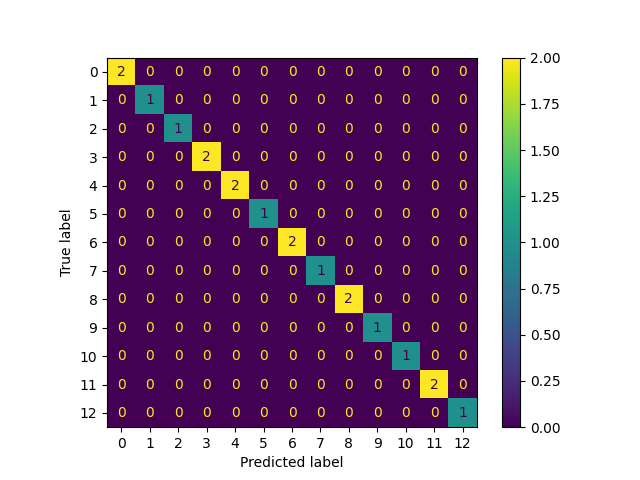
\includegraphics[width=0.45\textwidth]{dados/figuras/resultados/matrizes-confusao/gabor-brodatz-decision-tree.png} }}
    \qquad
    \subfloat[\centering MST]{{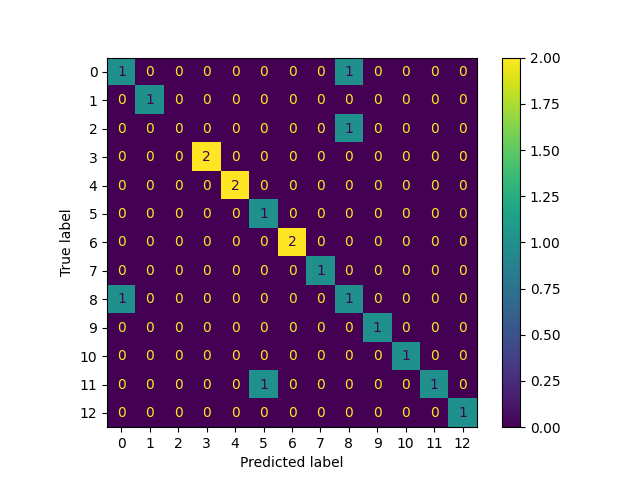
\includegraphics[width=0.45\textwidth]{dados/figuras/resultados/matrizes-confusao/mst-brodatz-decision-tree.png}}}
    \fonte{Autoria Própria.}
    \label{fig:uscSipiDecisionTreeMatrizConfusao}
\end{figure}

\begin{figure}[!h]
    \centering
    \caption{Matrizes de confusão para USC-SIPI \textit{Textures dataset} com uso de KNN}
    \subfloat[\centering Gabor]{{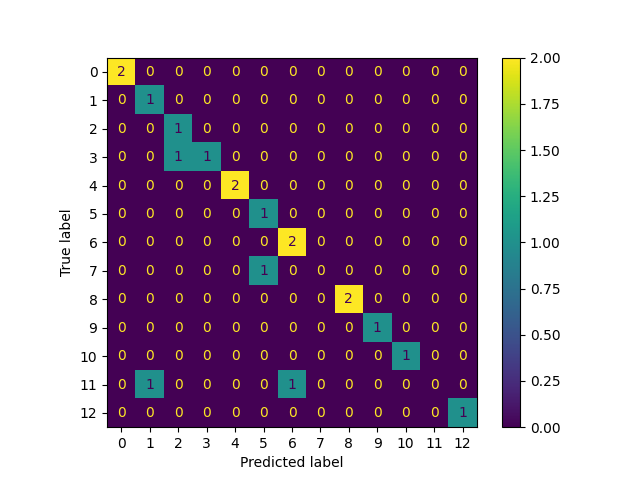
\includegraphics[width=0.45\textwidth]{dados/figuras/resultados/matrizes-confusao/gabor-brodatz-knn.png} }}
    \qquad
    \subfloat[\centering Haralick]{{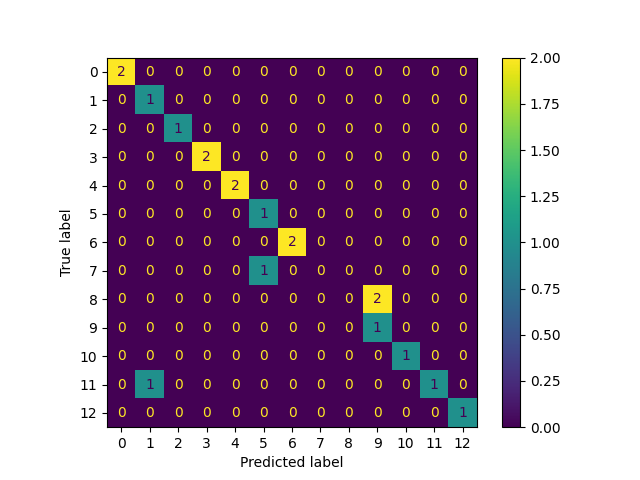
\includegraphics[width=0.45\textwidth]{dados/figuras/resultados/matrizes-confusao/haralick-brodatz-knn.png}}}
    \qquad
    \subfloat[\centering MST]{{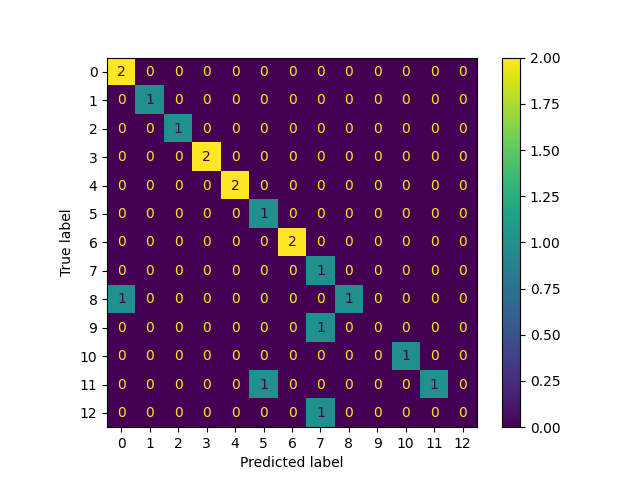
\includegraphics[width=0.45\textwidth]{dados/figuras/resultados/matrizes-confusao/mst-brodatz-knn.png}}}
    \fonte{Autoria Própria.}
    \label{fig:uscSipiKNNMatrizConfusao}
\end{figure}

\begin{figure}[!h]
    \centering
    \caption{Matrizes de confusão para USC-SIPI \textit{Textures dataset} com uso de \textit{Linear} SVC}
    \subfloat[\centering LBP]{{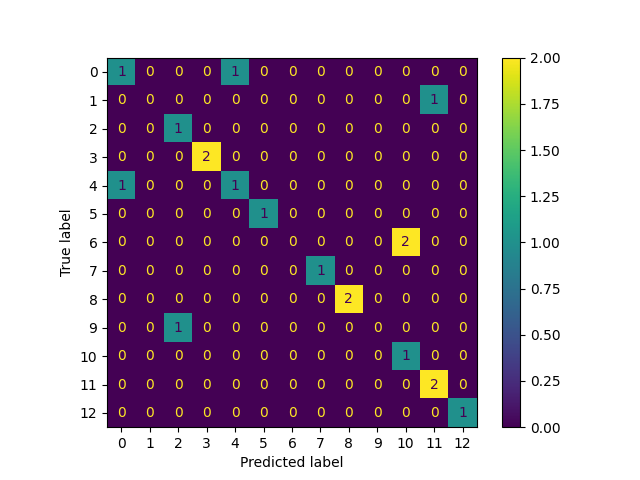
\includegraphics[width=0.45\textwidth]{dados/figuras/resultados/matrizes-confusao/lbp-brodatz-linear-svc.png} }}
    \qquad
    \subfloat[\centering MST]{{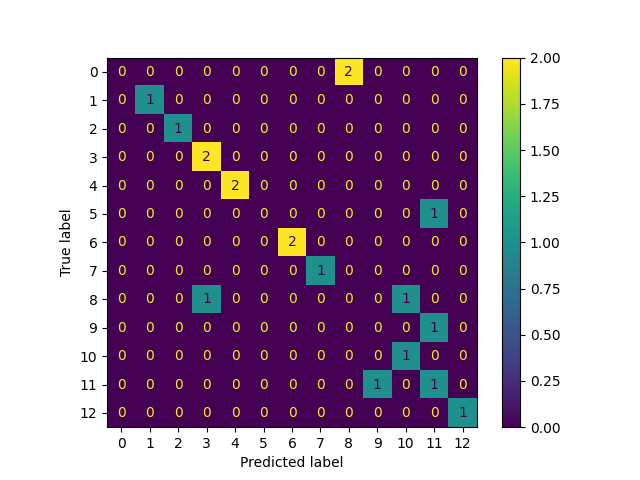
\includegraphics[width=0.45\textwidth]{dados/figuras/resultados/matrizes-confusao/mst-brodatz-linear-svc.png}}}
    \fonte{Autoria Própria.}
    \label{fig:uscSipiLinearSVCMatrizConfusao}
\end{figure}

\begin{figure}[!h]
    \centering
    \caption{Matrizes de confusão para USC-SIPI \textit{Textures dataset} com uso de SVC}
    \subfloat[\centering MST]{{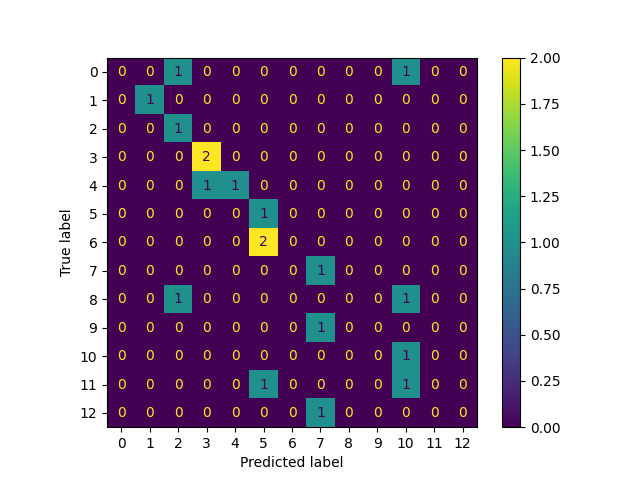
\includegraphics[width=0.45\textwidth]{dados/figuras/resultados/matrizes-confusao/mst-brodatz-svc.png}}}
    \qquad
    \subfloat[\centering Haralick]{{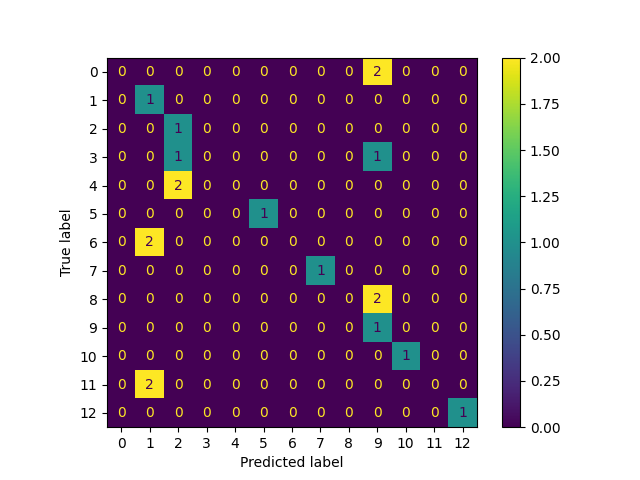
\includegraphics[width=0.45\textwidth]{dados/figuras/resultados/matrizes-confusao/haralick-brodatz-svc.png} }}
    \fonte{Autoria Própria.}
    \label{fig:uscSipiSVCMatrizConfusao}
\end{figure}

% Dataset Kylberg
\section{KYLBERG}
\label{sec:kylberg}

\par A partir dos testes realizados no \textit{dataset} Kylberg, foram estraídas as acurácias que estão disponíveis na \autoref{tab:kylbergAcuracias}. Através dos resultados pode-se observar que com o uso de \textit{Decision Tree} o extrator que obteve a melhor acurácia foi o LBP (93,20\%), seguido pelo Haralick (88,28\%) e pelo extrator proposto (88,06\%), respectivamente. Ao utilizar KNN, o extrator LBP apresentou novamente a melhor acurácia (96,21\%), seguido pelo MST (79,46\%). Com o algoritmo de aprendizado supervisionado \textit{Linear} SVC, o extrator LBP apresentou pela terceira vez o melhor resultado no \textit{dataset} (99,33\%), com o segundo lugar para o MST (68,75\%). Por fim, o SVC apresentou-se como o melhor resultado do extrator LBP (94,08\%), seguido por Tamura (64,17\%) e depois pelo extrator proposto (55,92\%). As matrizes de confusão para a comparação entre as melhores acurácias são expressas nas figuras \ref{fig:kylbergDecisionTreeMatrizConfusao}, \ref{fig:kylbergKNNMatrizConfusao}, \ref{fig:kylbergLinearSVCMatrizConfusao} e \ref{fig:kylbergSVCMatrizConfusao}.

\begin{table}[H]
    \centering
    \caption[Resultado das acurácias obtidas no \textit{dataset} Kylberg]{Resultado das acurácias obtidas no \textit{dataset} Kylberg
    \label{tab:kylbergAcuracias}}
    \begin{tabular}{rrrrrr}
        \toprule
            & Gabor (\%) & Haralick (\%) & LBP (\%) & Tamura (\%) & MST (\%) \\
        \midrule
            Decision Tree & 19,98 & 88,28 & 93,30 & 73,10 & 88,06 \\
            KNN & 18,64 & 46,21 & 96,21 & 59,38 & 79,46 \\
            Linear SVC & 9,71 & 5,69 & 99,33 & 26,34 & 68,75 \\
            SVC & 8,82 & 29,58 & 94,08 & 64,17 & 55,92 \\
        \bottomrule
    \end{tabular}
    \fonte{Autoria Própria.}
\end{table}


\begin{figure}[H]
    \centering
    \caption{Matrizes de confusão para o \textit{dataset} Kylberg com uso de \textit{Decision Tree}}
    \subfloat[\centering LBP]{{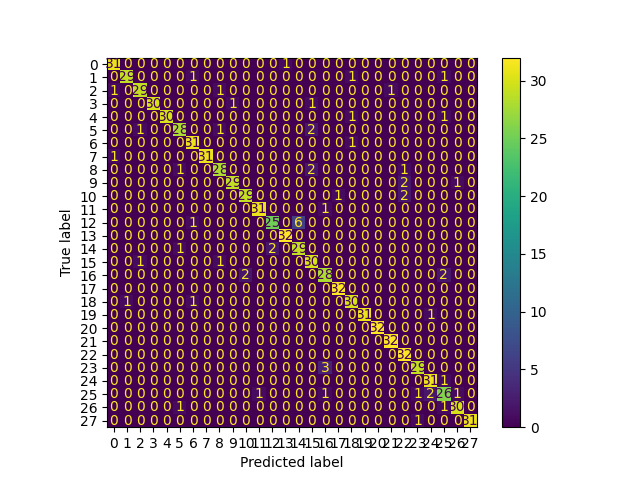
\includegraphics[width=0.45\textwidth]{dados/figuras/resultados/matrizes-confusao/lbp-kylberg-decision-tree.png}}}
    \qquad
    \subfloat[\centering Haralick]{{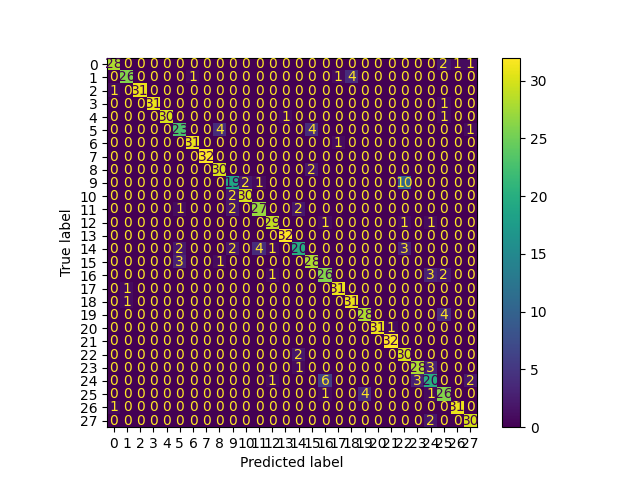
\includegraphics[width=0.45\textwidth]{dados/figuras/resultados/matrizes-confusao/haralick-kylberg-decision-tree.png} }}
    \qquad
    \subfloat[\centering MST]{{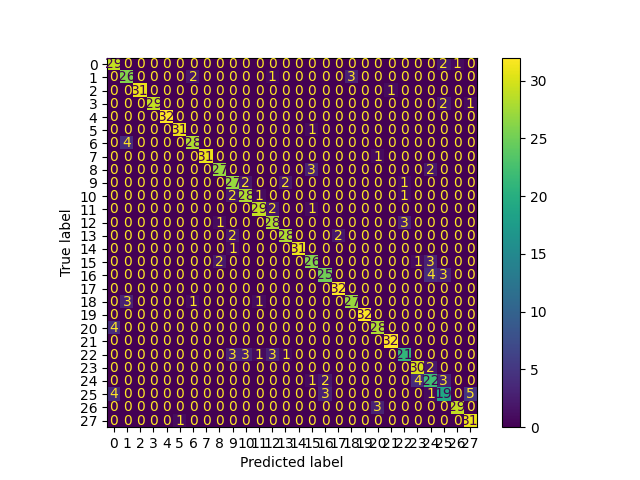
\includegraphics[width=0.45\textwidth]{dados/figuras/resultados/matrizes-confusao/mst-kylberg-decision-tree.png} }}
    \fonte{Autoria Própria.}
    \label{fig:kylbergDecisionTreeMatrizConfusao}
\end{figure}

\begin{figure}[H]
    \centering
    \caption{Matrizes de confusão para o \textit{dataset} Kylberg com uso de KNN}
    \subfloat[\centering LBP]{{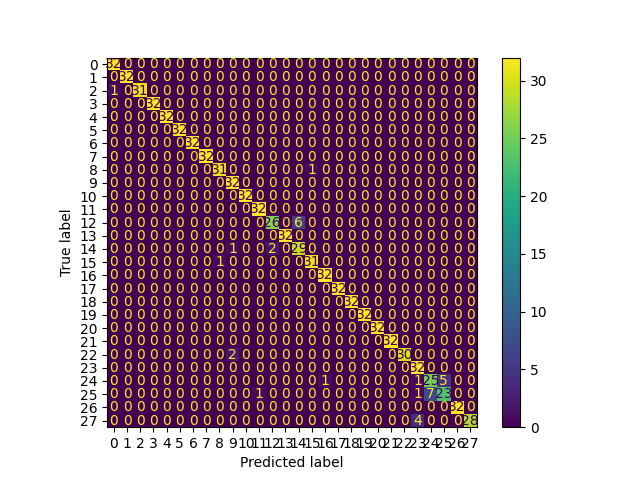
\includegraphics[width=0.45\textwidth]{dados/figuras/resultados/matrizes-confusao/lbp-kylberg-knn.png}}}
    \qquad
    \subfloat[\centering MST]{{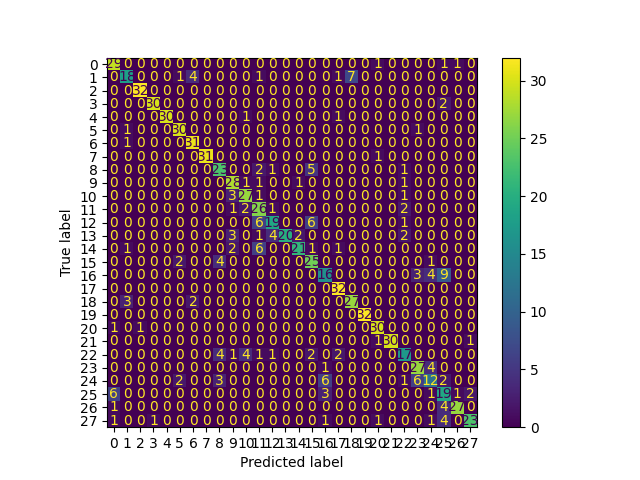
\includegraphics[width=0.45\textwidth]{dados/figuras/resultados/matrizes-confusao/mst-kylberg-knn.png} }}
    \fonte{Autoria Própria.}
    \label{fig:kylbergKNNMatrizConfusao}
\end{figure}


\begin{figure}[H]
    \centering
    \caption{Matrizes de confusão para o \textit{dataset} Kylberg com uso de \textit{Linear} SVC}
    \subfloat[\centering LBP]{{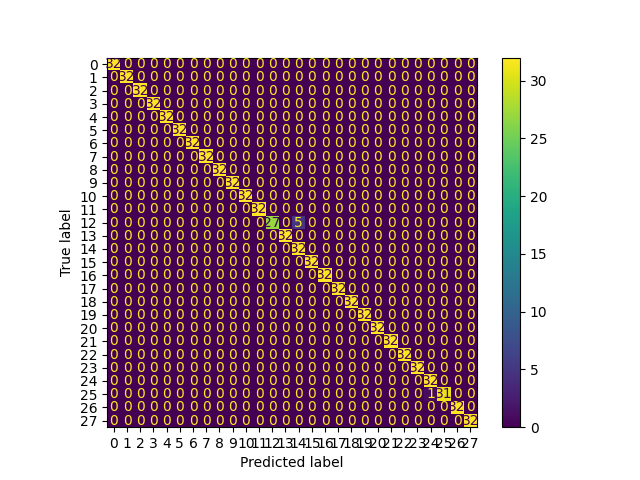
\includegraphics[width=0.45\textwidth]{dados/figuras/resultados/matrizes-confusao/lbp-kylberg-linear-svc.png}}}
    \qquad
    \subfloat[\centering MST]{{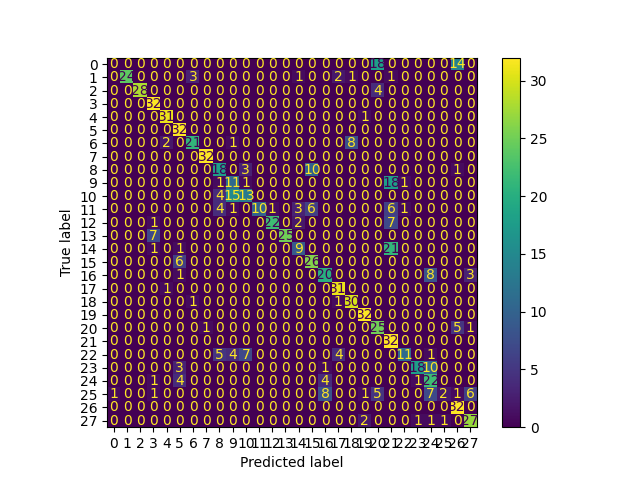
\includegraphics[width=0.45\textwidth]{dados/figuras/resultados/matrizes-confusao/mst-kylberg-linear-svc.png} }}
    \fonte{Autoria Própria.}
    \label{fig:kylbergLinearSVCMatrizConfusao}
\end{figure}

\begin{figure}[H]
    \centering
    \caption{Matrizes de confusão para o \textit{dataset} Kylberg com uso de SVC}
    \subfloat[\centering LBP]{{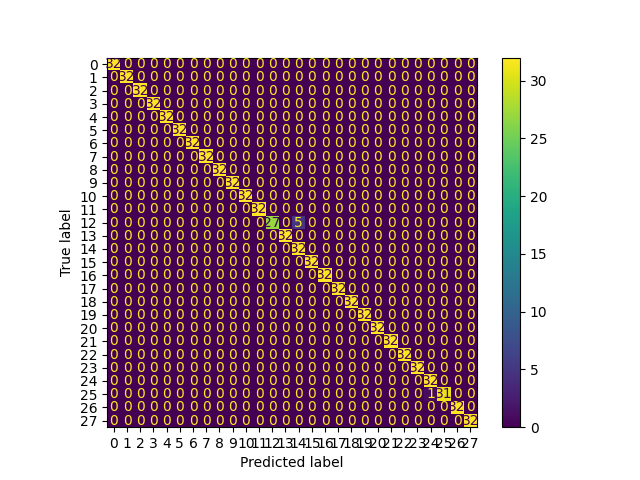
\includegraphics[width=0.45\textwidth]{dados/figuras/resultados/matrizes-confusao/lbp-kylberg-linear-svc.png}}}
    \qquad
    \subfloat[\centering Haralick]{{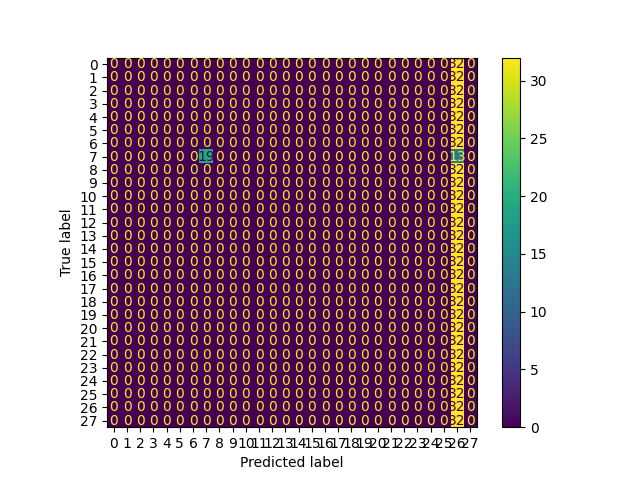
\includegraphics[width=0.45\textwidth]{dados/figuras/resultados/matrizes-confusao/haralick-kylberg-linear-svc.png} }}
    \qquad
    \subfloat[\centering MST]{{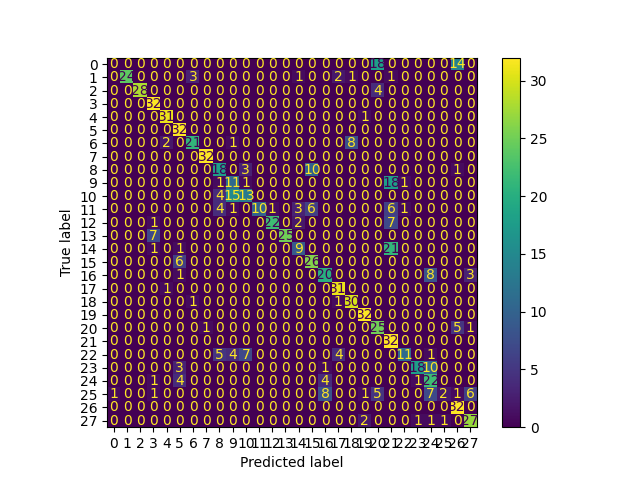
\includegraphics[width=0.45\textwidth]{dados/figuras/resultados/matrizes-confusao/mst-kylberg-linear-svc.png} }}
    \fonte{Autoria Própria.}
    \label{fig:kylbergSVCMatrizConfusao}
\end{figure}

% Dataset USPTex
\section{USPTEX}
\label{sec:usptex}

\par Os resultados das acurácias obtidas para os extratores e algoritmos de aprendizado supervisionado no \textit{dataset} USPtex estão descritos na \autoref{tab:USPtexAcuracias}. Com o Decision Tree, a maior acurácia corresponde ao extrator LBP (44.66\%), estando o algoritmo proposto na quarta posição (31,81\%). Ao utilizar KNN, o melhor extrator é o LBP (77,12\%), seguido do Tamura (30,28\%) e logo após o MST (19,61\%). Já com \textit{Linear} SVC, o melhor resultado se mantém com o extrator LBP (76,47\%), seguido pelo MST (13,51\%). Ao fim, utilizando SVC, o LBP se apresentou com a maior acurácia (46,19\%), após Tamura (24,84\%) e MST (10,24\%). Assim como exemplificado nos \textit{datasets} anteriores, nas figuras \ref{fig:usptexDecisionTreeMatrizConfusao}, \ref{fig:usptexKNNMatrizConfusao}, \ref{fig:usptexLinearSVCMatrizConfusao} e \ref{fig:usptexSVCMatrizConfusao} se encontram as comparações entre matrizes de confusão.

\begin{table}[H]
    \centering
    \caption[Resultado das acurácias obtidas no USPtex]{Resultado das acurácias obtidas no \textit{dataset} USPtex
    \label{tab:USPtexAcuracias}}
    \begin{tabular}{rrrrrr}
        \toprule
            & Gabor (\%) & Haralick (\%) & LBP (\%) & Tamura (\%) & MST (\%) \\
        \midrule
            Decision Tree & 20,92 & 42,05 & 44,66 & 32,90 & 31,81 \\
            KNN & 6,10 & 7,41 & 77,12 & 30,28 & 19,61 \\
            Linear SVC & 1,96 & 1,53 & 76,47 & 8,50 & 13,51 \\
            SVC & 6,10 & 6,10 & 46,19 & 24,84 & 10,24 \\
        \bottomrule
    \end{tabular}
    \fonte{Autoria Própria.}
\end{table}


\begin{figure}[H]
    \centering
    \caption{Matrizes de confusão para o \textit{dataset} USPtex com uso de \textit{Decision Tree}}
    \subfloat[\centering LBP]{{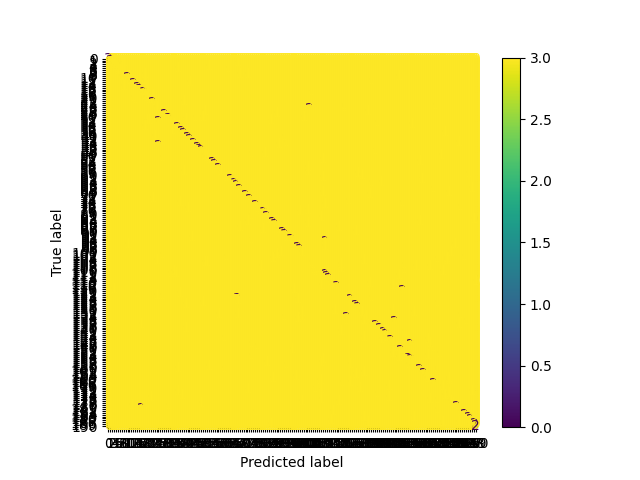
\includegraphics[width=0.45\textwidth]{dados/figuras/resultados/matrizes-confusao/lbp-usptex-decision-tree.png}}}
    \qquad
    \subfloat[\centering Haralick]{{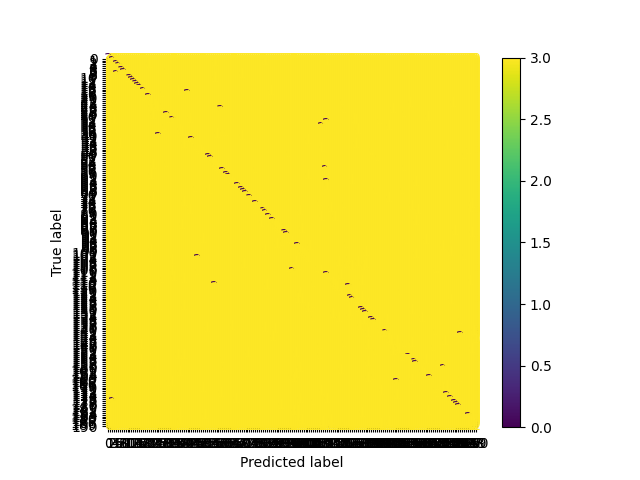
\includegraphics[width=0.45\textwidth]{dados/figuras/resultados/matrizes-confusao/haralick-usptex-decision-tree.png} }}
    \qquad
    \subfloat[\centering Tamura]{{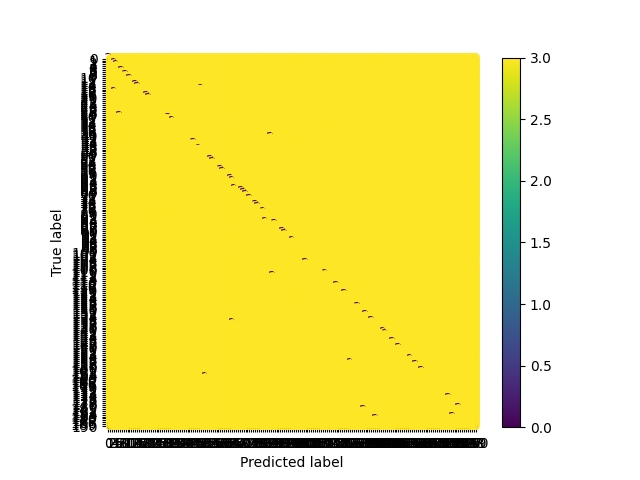
\includegraphics[width=0.45\textwidth]{dados/figuras/resultados/matrizes-confusao/tamura-usptex-decision-tree.png} }}
    \qquad
    \subfloat[\centering MST]{{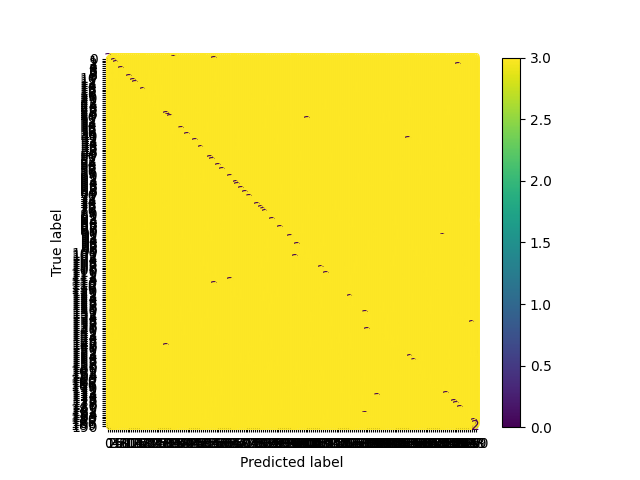
\includegraphics[width=0.45\textwidth]{dados/figuras/resultados/matrizes-confusao/mst-usptex-decision-tree.png} }}
    \fonte{Autoria Própria.}
    \label{fig:usptexDecisionTreeMatrizConfusao}
\end{figure}

\begin{figure}[H]
    \centering
    \caption{Matrizes de confusão para o \textit{dataset} USPtex com uso de KNN}
    \subfloat[\centering LBP]{{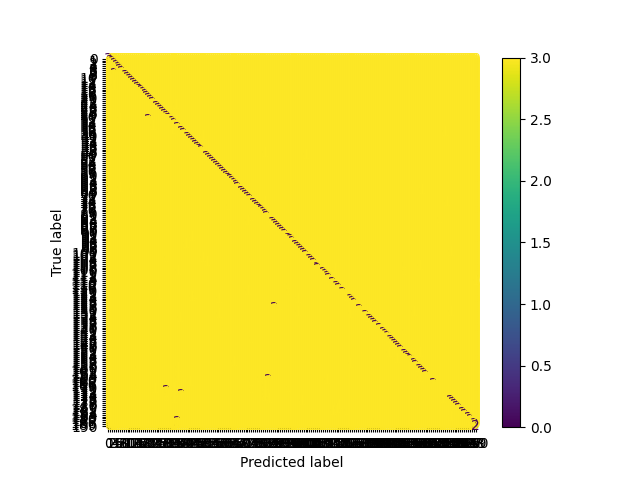
\includegraphics[width=0.45\textwidth]{dados/figuras/resultados/matrizes-confusao/lbp-usptex-knn.png}}}
    \qquad
    \subfloat[\centering Tamura]{{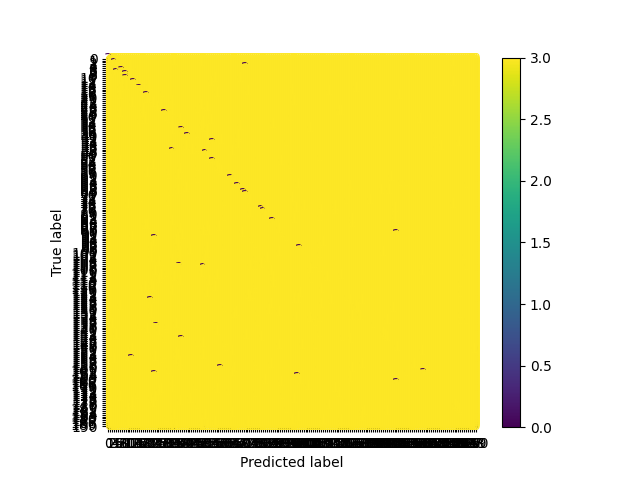
\includegraphics[width=0.45\textwidth]{dados/figuras/resultados/matrizes-confusao/mst-usptex-knn.png} }}
    \qquad
    \subfloat[\centering MST]{{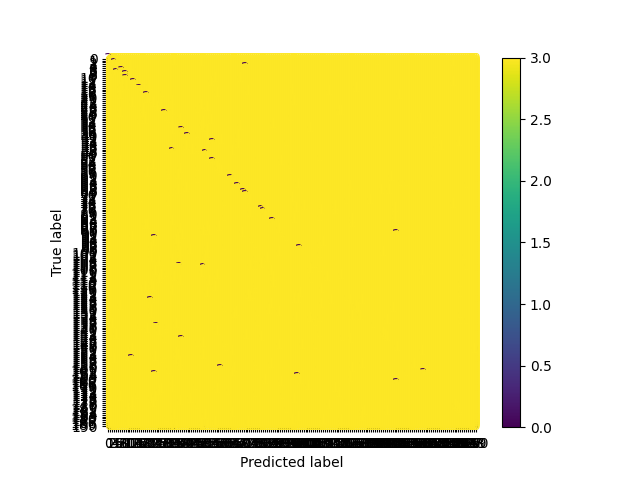
\includegraphics[width=0.45\textwidth]{dados/figuras/resultados/matrizes-confusao/mst-usptex-knn.png} }}
    \fonte{Autoria Própria.}
    \label{fig:usptexKNNMatrizConfusao}
\end{figure}

\begin{figure}[H]
    \centering
    \caption{Matrizes de confusão para o \textit{dataset} USPtex com uso de \textit{Linear} SVC}
    \subfloat[\centering LBP]{{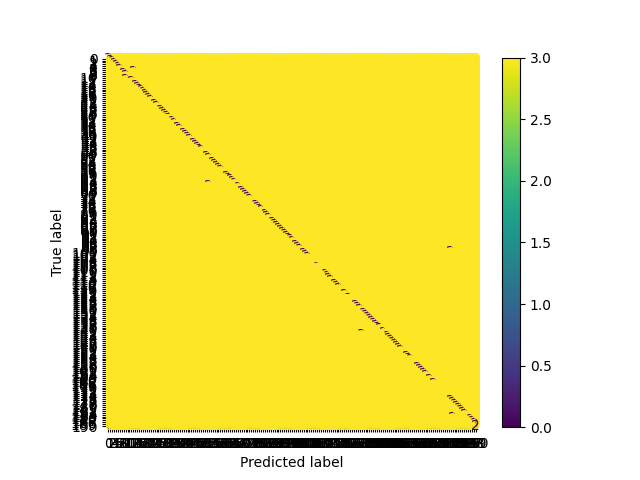
\includegraphics[width=0.45\textwidth]{dados/figuras/resultados/matrizes-confusao/lbp-usptex-linear-svc.png}}}
    \qquad
    \subfloat[\centering MST]{{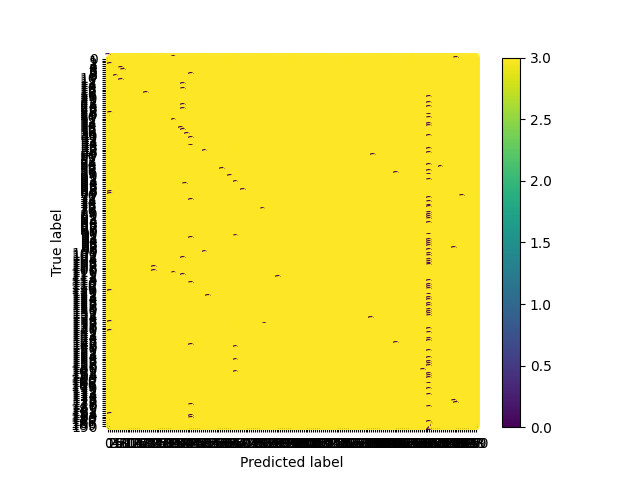
\includegraphics[width=0.45\textwidth]{dados/figuras/resultados/matrizes-confusao/mst-usptex-linear-svc.png} }}
    \fonte{Autoria Própria.}
    \label{fig:usptexLinearSVCMatrizConfusao}
\end{figure}

\begin{figure}[H]
    \centering
    \caption{Matrizes de confusão para o \textit{dataset} USPtex com uso de SVC}
    \subfloat[\centering LBP]{{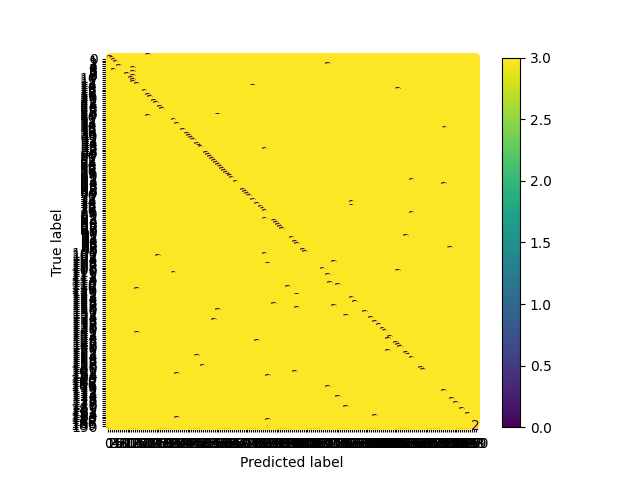
\includegraphics[width=0.45\textwidth]{dados/figuras/resultados/matrizes-confusao/lbp-usptex-svc.png}}}
    \qquad
    \subfloat[\centering MST]{{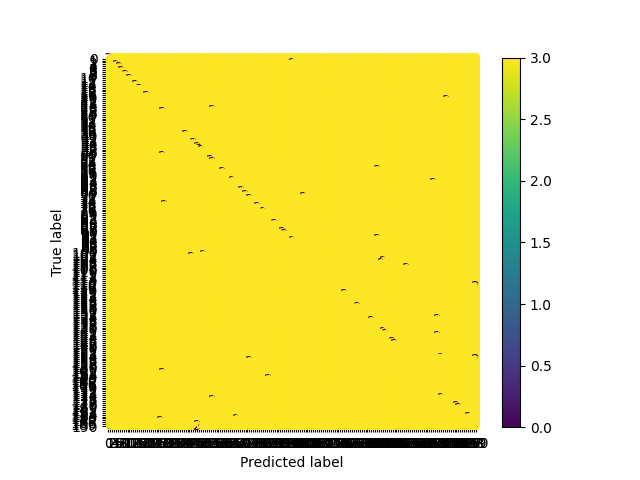
\includegraphics[width=0.45\textwidth]{dados/figuras/resultados/matrizes-confusao/tamura-usptex-svc.png} }}
    \qquad
    \subfloat[\centering MST]{{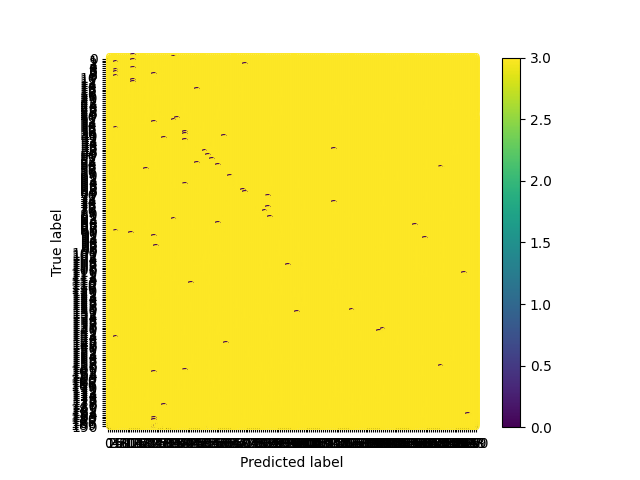
\includegraphics[width=0.45\textwidth]{dados/figuras/resultados/matrizes-confusao/mst-usptex-svc.png} }}
    \fonte{Autoria Própria.}
    \label{fig:usptexSVCMatrizConfusao}
\end{figure}

% Dataset VisTex
\section{VISTEX}
\label{sec:vistex}

\par Por fim, a tabela \autoref{tab:visTexAcuracias} representa uma comparação entre os valores obtidos das acurácias dos testes realizados no \textit{dataset} VisTex. Com o uso de \textit{Decision Tree} a maior acurácia foi do extrator MST (38,20\%), seguido por Gabor (29,41\%). Já o melhor resultado obtido com KNN, foi do extrator LBP, empatado com Tamura (29,41\%), seguido por Haralick que também ficou empatado com o MST (23,53\%). Para \textit{Linear} SVC, a maior acurácia foi do extrator LBP (52,94\%), seguido por Tamura (23,53\%) e posteriormente pelo MST (14,71\%). Para SVC, os extratores Gabor, Haralick e Tamura obtiveram a mesma acurácia de 26,47\%, seguido do LBP (23,47\%) e por fim MST (17,65\%). As figuras \ref{fig:vistexDecisionTreeMatrizConfusao}, \ref{fig:vistexKNNMatrizConfusao}, \ref{fig:vistexLinearSVCMatrizConfusao} e \ref{fig:vistexSVCMatrizConfusao}, exibem as matrizes de confusão obtidas durante os testes com o \textit{dataset} para fins de comparação.

\begin{table}[H]
    \centering
    \caption[Resultado das acurácias obtidas no VisTex]{Resultado das acurácias obtidas no \textit{dataset} VisTex.
    \label{tab:visTexAcuracias}}
    \begin{tabular}{rrrrrr}
        \toprule
            & Gabor (\%) & Haralick (\%) & LBP (\%) & Tamura (\%) & MST (\%) \\
        \midrule
            Decision Tree & 29,41 & 23,53 & 14,71 & 20,59 & 38,20 \\
            KNN & 20,59 & 23,53 & 29,41 & 29,41 & 23,53 \\
            Linear SVC & 11,76 & 5,88 & 52,94 & 23,53 & 14,71 \\
            SVC & 26,47 & 26,47 & 23,53 & 26,47 & 17,65 \\
        \bottomrule
    \end{tabular}
    \fonte{Autoria Própria}
\end{table}


\begin{figure}[H]
    \centering
    \caption{Matrizes de confusão para o \textit{dataset} VisTex com uso de \textit{Decision Tree}}
    \subfloat[\centering MST]{{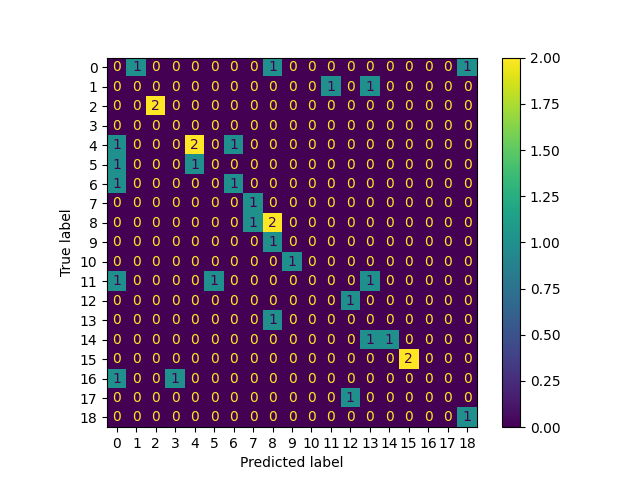
\includegraphics[width=0.45\textwidth]{dados/figuras/resultados/matrizes-confusao/mst-vistex-decision-tree.png} }}
    \qquad
    \subfloat[\centering Gabor]{{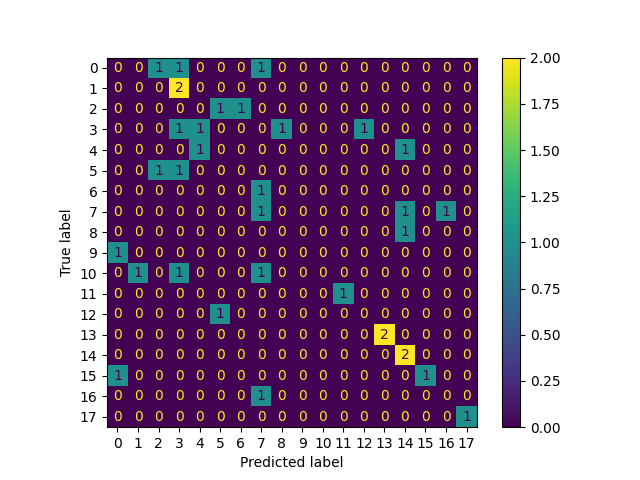
\includegraphics[width=0.45\textwidth]{dados/figuras/resultados/matrizes-confusao/gabor-vistex-decision-tree.png}}}
    \fonte{Autoria Própria.}
    \label{fig:vistexDecisionTreeMatrizConfusao}
\end{figure}

\begin{figure}[H]
    \centering
    \caption{Matrizes de confusão para o \textit{dataset} VisTex com uso de KNN}
    \subfloat[\centering LBP]{{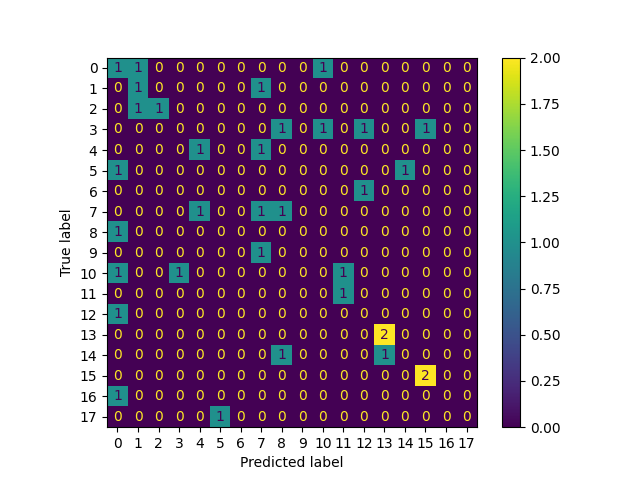
\includegraphics[width=0.45\textwidth]{dados/figuras/resultados/matrizes-confusao/lbp-vistex-knn.png}}}
    \qquad
    \subfloat[\centering Tamura]{{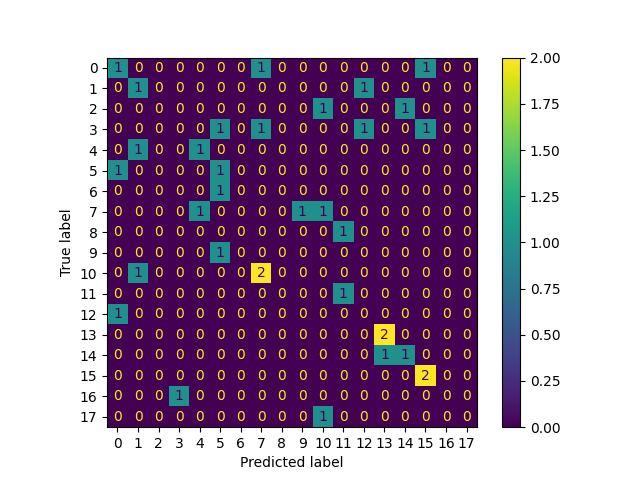
\includegraphics[width=0.45\textwidth]{dados/figuras/resultados/matrizes-confusao/tamura-vistex-knn.png}}}
    \qquad
    \subfloat[\centering MST]{{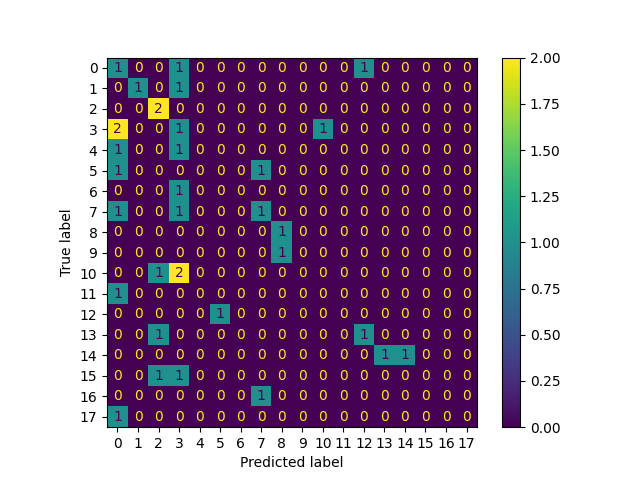
\includegraphics[width=0.45\textwidth]{dados/figuras/resultados/matrizes-confusao/mst-vistex-knn.png} }}
    \fonte{Autoria Própria.}
    \label{fig:vistexKNNMatrizConfusao}
\end{figure}

\begin{figure}[H]
    \centering
    \caption{Matrizes de confusão para o \textit{dataset} VisTex com uso de \textit{Linear} SVC}
    \subfloat[\centering LBP]{{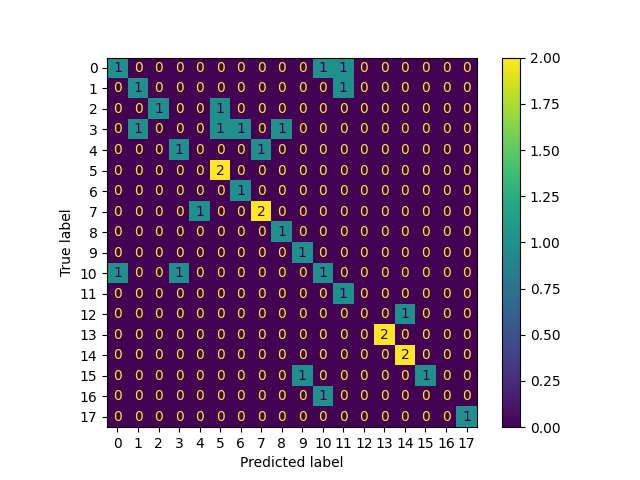
\includegraphics[width=0.45\textwidth]{dados/figuras/resultados/matrizes-confusao/lbp-vistex-linear-svc.png} }}
    \qquad
    \subfloat[\centering Tamura]{{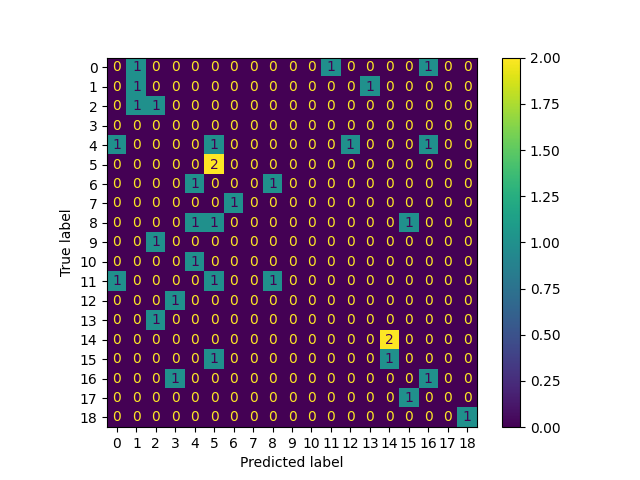
\includegraphics[width=0.45\textwidth]{dados/figuras/resultados/matrizes-confusao/tamura-vistex-linear-svc.png}}}
    \qquad
    \subfloat[\centering MST]{{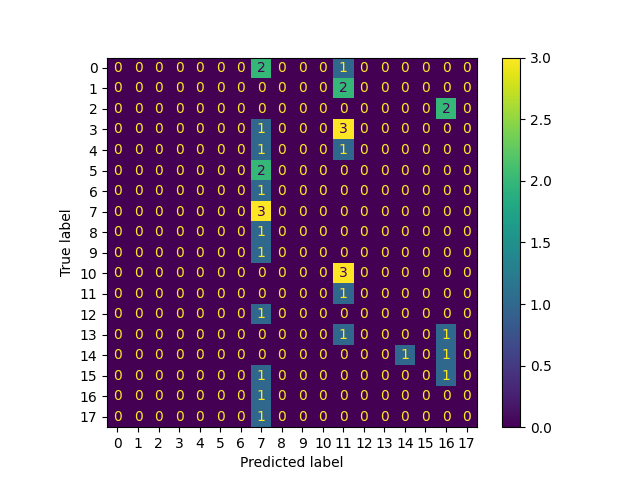
\includegraphics[width=0.45\textwidth]{dados/figuras/resultados/matrizes-confusao/mst-vistex-linear-svc.png}}}
    \fonte{Autoria Própria.}
    \label{fig:vistexLinearSVCMatrizConfusao}
\end{figure}

\begin{figure}[H]
    \centering
    \caption{Matrizes de confusão para o \textit{dataset} VisTex com uso de SVC}
    \subfloat[\centering Tamura]{{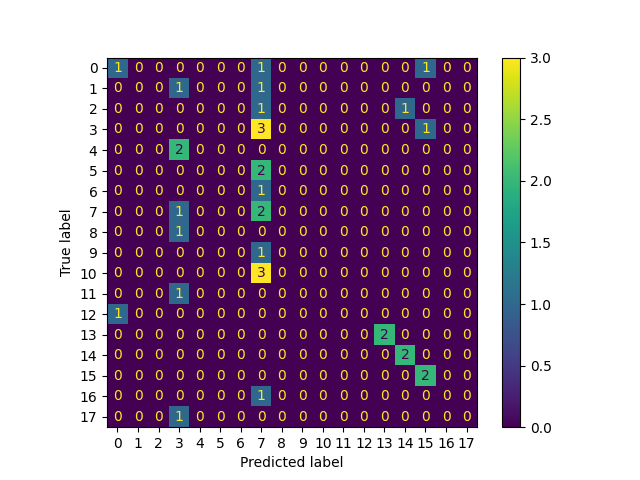
\includegraphics[width=0.45\textwidth]{dados/figuras/resultados/matrizes-confusao/tamura-vistex-svc.png} }}
    \qquad
    \subfloat[\centering Haralick]{{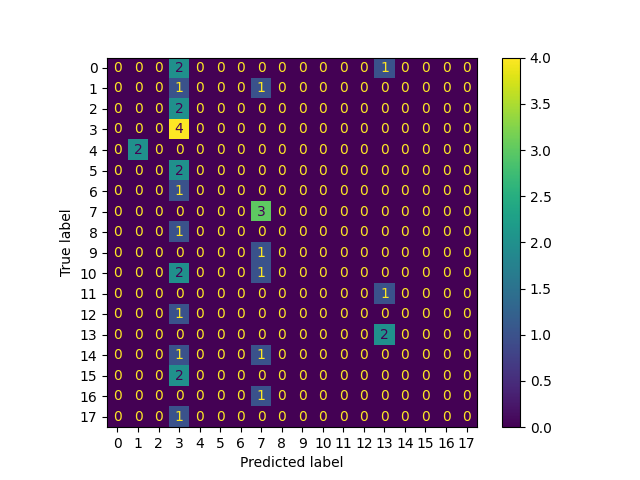
\includegraphics[width=0.45\textwidth]{dados/figuras/resultados/matrizes-confusao/haralick-vistex-svc.png}}}
    \qquad
    \subfloat[\centering Gabor]{{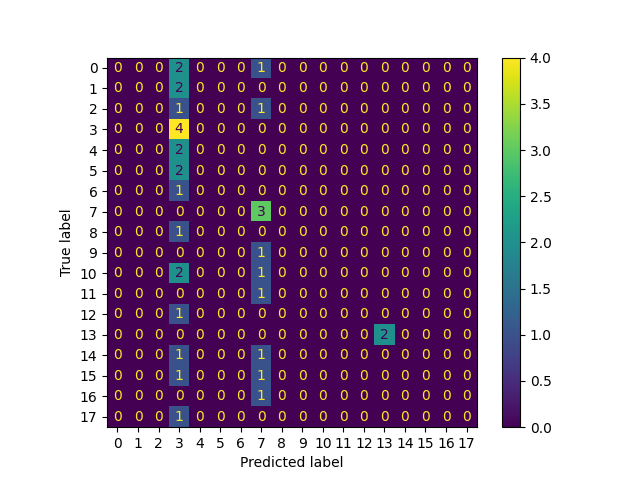
\includegraphics[width=0.45\textwidth]{dados/figuras/resultados/matrizes-confusao/gabor-vistex-svc.png}}}
    \qquad
    \subfloat[\centering MST]{{\includegraphics[width=0.45\textwidth]{dados/figuras/resultados/matrizes-confusao/mst-vistex-svc.png}}}
    \fonte{Autoria Própria.}
    \label{fig:vistexSVCMatrizConfusao}
\end{figure}

% Cronograma
% % CRONOGRAMA

\chapter{CRONOGRAMA}
\label{chap:cronograma}

\par Este capítulo tem como objetivo apresentar um cronograma para o futuro deste projeto. As fases, bem como suas atividades estão listadas logo em seguida e podem ser melhor observadas por meio da \autoref{tab:cronograma} e também através da \autoref{tab:cronograma-fases} as quais fazem uma relação entre atividades, fases e datas.

Vale ressaltar que as tabelas apresentam um mês e logo abaixo o número 1 e 2, o número 1 faz referência à primeira metade do mês e o número 2 à segunda metade\footnote{Exemplo: Dado o mês de novembro, o número 1 faz referência do dia 1 ao 15, já o número 2 faz referência do dia 16 ao 30.}.


\begin{enumerate}
    \item Correções
        \begin{enumerate}
            \item[1.1] Fazer as devidas correções neste documento, conforme detalhes apresentados pela banca e pelo orientador;
            \item[1.2] Verificar e validar correções.
        \end{enumerate}

    \item Preparação
        \begin{enumerate}
            \item[2.1] Definir premissas;
            \item[2.2] Definir módulos;
            \item[2.3] Verificar e validar;
            \item[2.4] Documentar e escrever sobre esta fase.
        \end{enumerate}

    \item Implementação
        \begin{enumerate}
            \item[3.1] Aprofundar conhecimentos em linguagem \textit{python};
            \item[3.2] Estudar novamente a documentação das bibliotecas e demais ferramentas, focando nos métodos que serão utilizados;
            \item[3.3] Iniciar a programação módulo $n$;
            \item[3.4] Testar o módulo $n$;
            \item[3.5] Documentar e escrever sobre esta fase.
        \end{enumerate}
        
    \item Integração
        \begin{enumerate}
            \item[4.1] Integrar os módulos da fase anterior;
            \item[4.2] Testar a integração;
            \item[4.3] Preparar o teste para a validação do algoritmo;
            \item[4.4] Testar o algoritmo;
            \item[4.5] Documentar e escrever sobre esta fase.
        \end{enumerate}
        
    \item Testes e comparações
        \begin{enumerate}
            \item[5.1] Estudar outros algoritmos de descrição de imagens;
            \item[5.2] Preparar testes entre o algoritmo obtido na fase anterior com os presentes na literatura;
            \item[5.3] Realizar testes;
            \item[5.4] Analisar resultados;
            \item[5.5] Verificar e validar;
            \item[5.6] Documentar e escrever sobre esta fase.
        \end{enumerate}
    
    \item Operação e manutenção
        \begin{enumerate}
            \item[6.1] Observar os resultados da etapa anterior e fazer as devidas modificações para a melhor eficiência do algoritmo;
            \item[6.2] Documentar e escrever sobre esta fase.
        \end{enumerate}
        
    \item Documentação
        \begin{enumerate}
            \item[7.1] Finalizar o documento referente ao Trabalho de Conclusão de Curso 2, utilizando da documentação das fases anteriores, além do documento produzido para o Trabalho de Conclusão de Curso 1;
            \item[7.2] Preparar apresentação.
        \end{enumerate}
        
\end{enumerate}

% Please add the following required packages to your document preamble:
% \usepackage[table,xcdraw]{xcolor}
% If you use beamer only pass "xcolor=table" option, i.e. \documentclass[xcolor=table]{beamer}
\begin{table}[H]
\centering
\caption{Cronograma do projeto por atividades.}
\label{tab:cronograma}
\resizebox{\textwidth}{!}{
\begin{tabular}{|l|l|l|l|l|l|l|l|l|l|l|l|l|l|l|l|l|}
\hline
\multicolumn{17}{|c|}{Cronograma}                                                                                                                                                                                                                                                                                                                                                                                                                                                                                                                     \\ \hline
Ano       & \multicolumn{4}{c|}{2019}                                                                                                        & \multicolumn{12}{c|}{2020}                                                                                                                                                                                                                                                                                                                                                                             \\ \hline
Mês       & \multicolumn{2}{c|}{Novembro}                                              & \multicolumn{2}{c|}{Dezembro}                       & \multicolumn{2}{c|}{Janeiro}                        & \multicolumn{2}{c|}{Fevereiro}                      & \multicolumn{2}{c|}{Março}                                                                        & \multicolumn{2}{c|}{Abril}                                                 & \multicolumn{2}{c|}{Maio}                           & \multicolumn{2}{c|}{Junho}                          \\ \hline
Atividade & \multicolumn{1}{c|}{1}   & \multicolumn{1}{c|}{2}                          & \multicolumn{1}{c|}{1}   & \multicolumn{1}{c|}{2}   & \multicolumn{1}{c|}{1}   & \multicolumn{1}{c|}{2}   & \multicolumn{1}{c|}{1}   & \multicolumn{1}{c|}{2}   & \multicolumn{1}{c|}{1}                          & \multicolumn{1}{c|}{2}                          & \multicolumn{1}{c|}{1}                          & \multicolumn{1}{c|}{2}   & \multicolumn{1}{c|}{1}   & \multicolumn{1}{c|}{2}   & \multicolumn{1}{c|}{1}   & \multicolumn{1}{c|}{2}   \\ \hline
1.1       & \cellcolor[HTML]{000000} &                                                 &                          &                          &                          &                          &                          &                          &                                                 &                                                 &                                                 &                          &                          &                          &                          &                          \\ \hline
1.2       & \cellcolor[HTML]{000000} &                                                 &                          &                          &                          &                          &                          &                          &                                                 &                                                 &                                                 &                          &                          &                          &                          &                          \\ \hline
2.1       &                          & \cellcolor[HTML]{000000}{\color[HTML]{000000} } &                          &                          &                          &                          &                          &                          &                                                 &                                                 &                                                 &                          &                          &                          &                          &                          \\ \hline
2.2       &                          & \cellcolor[HTML]{000000}                        &                          &                          &                          &                          &                          &                          &                                                 &                                                 &                                                 &                          &                          &                          &                          &                          \\ \hline
2.3       &                          & \cellcolor[HTML]{000000}                        &                          &                          &                          &                          &                          &                          &                                                 &                                                 &                                                 &                          &                          &                          &                          &                          \\ \hline
2.4       &                          & \cellcolor[HTML]{000000}                        &                          &                          &                          &                          &                          &                          &                                                 &                                                 &                                                 &                          &                          &                          &                          &                          \\ \hline
3.1       &                          &                                                 & \cellcolor[HTML]{000000} &                          &                          &                          &                          &                          &                                                 &                                                 &                                                 &                          &                          &                          &                          &                          \\ \hline
3.2       &                          &                                                 & \cellcolor[HTML]{000000} &                          &                          &                          &                          &                          &                                                 &                                                 &                                                 &                          &                          &                          &                          &                          \\ \hline
3.3       &                          &                                                 & \cellcolor[HTML]{000000} & \cellcolor[HTML]{000000} & \cellcolor[HTML]{000000} & \cellcolor[HTML]{000000} &                          &                          &                                                 &                                                 &                                                 &                          &                          &                          &                          &                          \\ \hline
3.4       &                          &                                                 & \cellcolor[HTML]{000000} & \cellcolor[HTML]{000000} & \cellcolor[HTML]{000000} & \cellcolor[HTML]{000000} &                          &                          &                                                 &                                                 &                                                 &                          &                          &                          &                          &                          \\ \hline
3.5       &                          &                                                 &                          &                          &                          & \cellcolor[HTML]{000000} &                          &                          &                                                 &                                                 &                                                 &                          &                          &                          &                          &                          \\ \hline
4.1       &                          &                                                 &                          &                          &                          &                          & \cellcolor[HTML]{000000} &                          &                                                 &                                                 &                                                 &                          &                          &                          &                          &                          \\ \hline
4.2       &                          &                                                 &                          &                          &                          &                          & \cellcolor[HTML]{000000} &                          &                                                 &                                                 &                                                 &                          &                          &                          &                          &                          \\ \hline
4.3       &                          &                                                 &                          &                          &                          &                          & \cellcolor[HTML]{000000} &                          &                                                 &                                                 &                                                 &                          &                          &                          &                          &                          \\ \hline
4.4       &                          &                                                 &                          &                          &                          &                          & \cellcolor[HTML]{000000} &                          &                                                 &                                                 &                                                 &                          &                          &                          &                          &                          \\ \hline
4.5       &                          &                                                 &                          &                          &                          &                          & \cellcolor[HTML]{000000} &                          &                                                 &                                                 &                                                 &                          &                          &                          &                          &                          \\ \hline
5.1       &                          &                                                 &                          &                          &                          &                          &                          & \cellcolor[HTML]{000000} &                                                 &                                                 &                                                 &                          &                          &                          &                          &                          \\ \hline
5.2       &                          &                                                 &                          &                          &                          &                          &                          & \cellcolor[HTML]{000000} &                                                 &                                                 &                                                 &                          &                          &                          &                          &                          \\ \hline
5.3       &                          &                                                 &                          &                          &                          &                          &                          &                          & \cellcolor[HTML]{000000}{\color[HTML]{000000} } &                                                 &                                                 &                          &                          &                          &                          &                          \\ \hline
5.4       &                          &                                                 &                          &                          &                          &                          &                          &                          & \cellcolor[HTML]{000000}{\color[HTML]{000000} } &                                                 &                                                 &                          &                          &                          &                          &                          \\ \hline
5.5       &                          &                                                 &                          &                          &                          &                          &                          &                          & \cellcolor[HTML]{000000}{\color[HTML]{000000} } &                                                 &                                                 &                          &                          &                          &                          &                          \\ \hline
5.6       &                          &                                                 &                          &                          &                          &                          &                          &                          & \cellcolor[HTML]{000000}{\color[HTML]{000000} } &                                                 &                                                 &                          &                          &                          &                          &                          \\ \hline
6.1       &                          &                                                 &                          &                          &                          &                          &                          &                          &                                                 & \cellcolor[HTML]{000000}{\color[HTML]{000000} } & \cellcolor[HTML]{000000}{\color[HTML]{000000} } & \cellcolor[HTML]{000000} & \cellcolor[HTML]{000000} &                          &                          &                          \\ \hline
6.2       &                          &                                                 &                          &                          &                          &                          &                          &                          &                                                 & \cellcolor[HTML]{000000}{\color[HTML]{000000} } & \cellcolor[HTML]{000000}{\color[HTML]{000000} } & \cellcolor[HTML]{000000} & \cellcolor[HTML]{000000} &                          &                          &                          \\ \hline
7.1       &                          &                                                 &                          &                          &                          &                          &                          &                          &                                                 &                                                 &                                                 & \cellcolor[HTML]{000000} & \cellcolor[HTML]{000000} & \cellcolor[HTML]{000000} & \cellcolor[HTML]{000000} &                          \\ \hline
7.2       &                          &                                                 &                          &                          &                          &                          &                          &                          &                                                 &                                                 &                                                 &                          &                          & \cellcolor[HTML]{000000} & \cellcolor[HTML]{000000} & \cellcolor[HTML]{000000} \\ \hline
\end{tabular}
}
\end{table}

Uma visão mais resumida e menos detalhada pode ser vista na \autoref{tab:cronograma-fases}, estando esta organizada através das fases do projeto, definidas no início deste \autoref{chap:cronograma}.

% Please add the following required packages to your document preamble:
% \usepackage[table,xcdraw]{xcolor}
% If you use beamer only pass "xcolor=table" option, i.e. \documentclass[xcolor=table]{beamer}
\begin{table}[H]
\centering
\caption{Cronograma do projeto por fases.}
\label{tab:cronograma-fases}
\resizebox{\textwidth}{!}{
\begin{tabular}{|l|l|l|l|l|l|l|l|l|l|l|l|l|l|l|l|l|}
\hline
\multicolumn{17}{|c|}{Cronograma}                                                                                                                                                                                                                                                                                                                                                                                                                    \\ \hline
Ano  & \multicolumn{4}{c|}{2019}                                                                                 & \multicolumn{12}{c|}{2020}                                                                                                                                                                                                                                                                                                        \\ \hline
Mês  & \multicolumn{2}{c|}{Novembro}                       & \multicolumn{2}{c|}{Dezembro}                       & \multicolumn{2}{c|}{Janeiro}                        & \multicolumn{2}{c|}{Fevereiro}                      & \multicolumn{2}{c|}{Março}                          & \multicolumn{2}{c|}{Abril}                          & \multicolumn{2}{c|}{Maio}                           & \multicolumn{2}{c|}{Junho}                          \\ \hline
Fase & \multicolumn{1}{c|}{1}   & \multicolumn{1}{c|}{2}   & \multicolumn{1}{c|}{1}   & \multicolumn{1}{c|}{2}   & \multicolumn{1}{c|}{1}   & \multicolumn{1}{c|}{2}   & \multicolumn{1}{c|}{1}   & \multicolumn{1}{c|}{2}   & \multicolumn{1}{c|}{1}   & \multicolumn{1}{c|}{2}   & \multicolumn{1}{c|}{1}   & \multicolumn{1}{c|}{2}   & \multicolumn{1}{c|}{1}   & \multicolumn{1}{c|}{2}   & \multicolumn{1}{c|}{1}   & \multicolumn{1}{c|}{2}   \\ \hline
1    & \cellcolor[HTML]{000000} &                          &                          &                          &                          &                          &                          &                          &                          &                          &                          &                          &                          &                          &                          &                          \\ \hline
2    &                          & \cellcolor[HTML]{000000} &                          &                          &                          &                          &                          &                          &                          &                          &                          &                          &                          &                          &                          &                          \\ \hline
3    &                          &                          & \cellcolor[HTML]{000000} & \cellcolor[HTML]{000000} & \cellcolor[HTML]{000000} & \cellcolor[HTML]{000000} &                          &                          &                          &                          &                          &                          &                          &                          &                          &                          \\ \hline
4    &                          &                          &                          &                          &                          &                          & \cellcolor[HTML]{000000} &                          &                          &                          &                          &                          &                          &                          &                          &                          \\ \hline
5    &                          &                          &                          &                          &                          &                          &                          & \cellcolor[HTML]{000000} & \cellcolor[HTML]{000000} &                          &                          &                          &                          &                          &                          &                          \\ \hline
6    &                          &                          &                          &                          &                          &                          &                          &                          &                          & \cellcolor[HTML]{000000} & \cellcolor[HTML]{000000} & \cellcolor[HTML]{000000} & \cellcolor[HTML]{000000} &                          &                          &                          \\ \hline
7    &                          &                          &                          &                          &                          &                          &                          &                          &                          &                          &                          & \cellcolor[HTML]{000000} & \cellcolor[HTML]{000000} & \cellcolor[HTML]{000000} & \cellcolor[HTML]{000000} & \cellcolor[HTML]{000000} \\ \hline
\end{tabular}
}
\end{table}
% Considerações Finais
% % CONCLUSÃO--------------------------------------------------------------------

\chapter{CONSIDERAÇÕES FINAIS}
\label{chap:consideracoesFinais}

\par Por tanto, a proposta deste trabalho é definir e especificar um projeto que procura desenvolver uma nova maneira, de descrever texturas em uma imagem, por meio da utilização de grafos e também de árvores geradoras mínimas.
\par Como observado, a descrição é uma parte importante do processamento digital de imagens, pois é capaz de identificar padrões em um objeto selecionado pela etapa de segmentação.
\par Sendo assim, é esperado que com a conclusão do algoritmo, este seja capaz de descrever texturas em imagens digitais de forma a ser mais eficaz e/ou eficiente quando comparado a outros algoritmos já presentes na literatura. Além disso, espera-se que com este documento, devidamente atualizado após a conclusão, possa ser utilizado para futuras melhorias no algoritmo e também em novas abordagens.

\section{TRABALHOS FUTUROS}
\label{sec:trabalhos-futuros}

\par É de conhecimento que para este estudo ser bem-sucedido é necessário seguir a metodologia, descrita na \autoref{sec:metodo}, em conjunto com o cronograma apresentado no \autoref{chap:cronograma}.
\par Dessa forma, a partir do mês de novembro de 2019 será dada continuidade nos trabalhos descritos neste documento, bem como anteriormente apresentados, e serão devidamente finalizados em junho de 2020.

% Conclusão
\chapter{CONCLUSÃO}
\label{chap:conclusao}

\par A partir das discussões propostas por este trabalho e dos resultados obtidos é possível afirmar que o método de extração de características com árvore geradora mínima se mostra eficaz e pode ser utilizado para a caracterização de texturas de imagens.

\par Ao observar o \textit{dataset} USC-SIPI \textit{Textures}, pode-se concluir que o extrator proposto, MST, obteve resultados tão bons quanto os extratores comparados, sendo capaz até mesmo de supera-los quando utilizado com SVC. Com o \textit{dataset} de Kylberg, os resultados não foram muito diferentes, apesar do extrator LBP se manter como melhor em todos os cenários, o extrator proposto se mantém em segundo lugar em quase todos os testes. Porém, o MST não apresentou resultados animadores durante os testes com o \textit{dataset} USPtex, exceto pelo extrator LBP, os outros também não apresentaram resultados significantes. Por fim, para o \textit{dataset} VisTex, nenhum extrator obteve uma acurácia maior que 55\% em todos os tipos testes, sendo o extrator proposto mantido em segundo lugar e em primeiro quando utilizado com \textit{Decision Tree}. Mais informações sobre os resultados estão disponíveis no \textit{github}\footnote{\url{https://github.com/felipeseolin/image-texture-classification-tests}}, assim com o código fonte do extrator\footnote{\url{https://github.com/felipeseolin/image-texture-classification}}.

\par Apesar de existirem casos em que outros algoritmos obtiveram melhores resultados de acurácia e matriz de confusão, o extrator proposto foi capaz de coletar com eficácia as informações necessárias para o reconhecimento texturas de imagens com um número reduzido de características. A \autoref{tab:extratorXqtdCaracteristicas}, apresenta a relação entre os extratores e número de características que cada um deles utiliza.

\begin{table}[H]
    \centering
    \caption[Extratores e quantidades de características]{Extratores e quantidades de características
    \label{tab:extratorXqtdCaracteristicas}}
    \begin{tabular}{cc}
        \toprule
            Extrator & Números de características \\
        \midrule
            Gabor & 60 \\
            Haralick & 14 \\
            LBP & 256 \\
            Tamura & 18 \\
            MST & 5 \\
        \bottomrule
    \end{tabular}
    \fonte{Autoria Própria.}
\end{table}


% \par (REVER) É importante destacar que medidas de custo computacional e tempo de execução não foram levadas em consideração neste trabalho, pois o processo de extração de características de uma imagem (descrição) é, em geral, um processo custoso e demorado, sendo sempre realizado de forma prévia.
% \par No entanto, é importante ressaltar que o algoritmo proposto apresentou um tempo relativamente alto, quando comparado aos outros algoritmos, o que faz com que ele precise ser aperfeiçoado e otimizado. Isto pode ser feito reduzindo o uso de algumas bibliotecas que fornecem objetos e funções não necessárias, mas mesmo assim o processamento é executado. Como exemplo, a biblioteca igraph a qual retorna sempre um objeto Graph como resultado, sendo que só é necessário um array com os valores das arestas da MST.

\par Com o intuito de fornecer maiores comparações com os extratores e estabelecer melhores métricas, foram realizados testes sobre o tempo de execução com a \autoref{fig:tempoExecucao} retirada do \textit{dataset} USC-SIPI \textit{Textures}. Vale ressaltar que o computador utilizado possui processador Intel Core i5-8250U, CPU 1.60GHz 1.80GHz, 8GB de memória RAM instalada e 7.90GB utilizável, além de com o sistema operacional Windows 11 arquitetura \textit{64-bits}.

\pagebreak 

\begin{figure}[!h]
    \centering
    \caption{Imagem utilizada para calcular o tempo de execução.}
    \includegraphics[width=0.5\textwidth]{./dados/figuras/testeExecucao.png}
    \fonte{\citeonline{weber1997usc}}
    \label{fig:tempoExecucao}
\end{figure}

\par A partir disto, na \autoref{tab:extratorXtempoExecucao} foram descritos os tempos de execução do extrator proposto em relação com os outros testados neste trabalho. Neste sentido, pode-se observar que o MST obteve um tempo de execução maior quando comparados com os outros, sendo que o extrator com o menor tempo de execução foi o Haralick. 

\begin{table}[H]
    \centering
    \caption[Extratores e tempo de execução]{Extratores e tempo de execução
    \label{tab:extratorXtempoExecucao}}
    \begin{tabular}{cc}
        \toprule
            Extrator & Tempo de execução em segundos \\
        \midrule
            Gabor & 1,13s \\
            Haralick & 1,03s \\
            LBP & 1,28s \\
            Tamura & 2,35s \\
            MST & 3,26s \\
        \bottomrule
    \end{tabular}
    \fonte{Autoria Própria.}
\end{table}


\par Dessa forma, nota-se que o extrator deve melhorar sua performe, de forma a otimizar o tempo de execução, isto seria possível reduzindo o uso de bibliotecas que podem carregar consigo funções além do necessário, como a biblioteca \textit{igraph}, a qual retorna sempre um objeto \textit{Graph} como resultado, sendo necessário apenas um \textit{array} com os valores das arestas da MST.

\par Por fim, pode-se concluir que o uso de grafos e de árvore geradora mínima, soluções já utilizadas em outros contextos de problemas na computação, mostra-se mais uma vez eficaz, agora para o reconhecimento de texturas. Além disso, vale ressaltar que nenhum descritor obteve resultados absolutamente melhores em todos os casos. Na maior parte, o algoritmo proposto se manteve como melhor, ou segundo melhor, em relação a acurácia. Estes dados provam que a criação de novos descritores é valida e necessária para o aprimoramento da área de processamento de imagens digitais.

\section{TRABALHOS FUTUROS}
\label{sec:trabalhosFuturos}

\par Em trabalhos futuros, o extrator pode ser comparado a outros extratores de textura presentes na literatura, principalmente aqueles que utilizam grafos como método principal. Também é possível mudar alguns parâmetros durante o aprendizado supervisionado, como a semente, divisão entre teste e treino, normalização e outros algoritmos.

\par Mudar a forma que os pesos das arestas são gerados e adicionar características, também poderiam aumentar a acurácia do algoritmo durante os testes, porém deve-se levar em conta o tempo de execução e custo computacional de tais mudanças. Neste sentido, a aplicação de técnicas antes mesmo do desenvolvimento do algoritmo, como a utilização de \textit{superpixels} pode reduzir o custo computacional e melhorar a performance do extrator.

\par Além disso, seria interessante aprimorar o extrator no contexto de suporte a imagens com cores RGB. Um caminho possíveis para isto é a expansão do número de ligações dos \textit{pixels}, assim um \textit{pixel} não se ligaria apenas com os \textit{pixels} de sua camada, mas também da camada inferior a este.

\par Por fim, a partir de todas as discussões levantadas por este trabalho, pode-se concluir que o desenvolvimento de diferentes trabalhos e abordagens do processamento de imagens digitais tem grande aceitação e espaço para crescimento, por isso se fazem necessárias para a evolução da área.


% INSERE ELEMENTOS PÓS-TEXTUAIS
\postextual
% Referências
% REFERÊNCIAS------------------------------------------------------------------

% Carrega o arquivo "base-referencias.bib" e extrai automaticamente as referências citadas

\bibliography{./base-referencias}
\bibliographystyle{abntex2-alf} % Define o estilo ABNT para formatar a lista de referências
% OBSERVAÇÕES------------------------------------------------------------------
% Este arquivo não precisa ser alterado.

% Apêndices
% APÊNDICES--------------------------------------------------------------------

\begin{apendicesenv}
\partapendices

% Primeiro apêndice------------------------------------------------------------
\chapter{Resultados detalhados dos testes}
\label{chap:apendiceResultados}

% \section{Extrator Gabor com \textit{dataset} USC-SIPI \textit{Textures}}

% \subsection{Decision Tree}

% \begin{figure}[!h]
%     \centering
%     \caption{Matriz de confusão para o extrator Gabor com uso de \textit{Decision Tree} para o \textit{dataset} USC-SIPI \textit{Textures}.}
%     \includegraphics[width=0.7\textwidth]{./dados/figuras/resultados/matrizes-confusao/gabor-brodatz-decision-tree.png}
%     \fonte{Autoria Própria}
%     \label{fig:tempoExecucao}
% \end{figure}

% \par Resultados

\end{apendicesenv}


\end{document}
